\documentclass{mcmthesis}
\mcmsetup{CTeX = false,   % 使用 CTeX 套装时,设置为 true
        tcn = 86483, problem = E,
        sheet = true, titleinsheet = true, keywordsinsheet = false,
        titlepage = false, abstract = true}
\usepackage{palatino}
\usepackage{booktabs}
\usepackage{lipsum}
\usepackage{float}
\usepackage{wrapfig}
\usepackage{geometry}%页面设置  
\usepackage{graphics}%图片设置  
% 这两行可以让点击图片引用显示整个图片,而不是只有字
\usepackage{caption}%注释设置
\captionsetup{hypcap=true}

\title{Is my country fragile?}
\author{\small \href{http://www.latexstudio.net/}
  {\includegraphics[width=7cm]{mcmthesis-logo}}}
\date{\today}

\renewcommand\arraystretch{1.05}
\newcolumntype{I}{!{\vrule width 1.2pt}}
\newlength\savedwidth
\newcommand\whline{\noalign{\global\savedwidth\arrayrulewidth
                            \global\arrayrulewidth 3pt}%
                   \hline
                   \noalign{\global\arrayrulewidth\savedwidth}}
\newlength\savewidth
\newcommand\shline{\noalign{\global\savewidth\arrayrulewidth
                            \global\arrayrulewidth 1.5pt}%
                   \hline
                   \noalign{\global\arrayrulewidth\savewidth}}
% 让引用变成右上标形式,使用\upcite
\newcommand{\upcite}[1]{\textsuperscript{\textsuperscript{\cite{#1}}}}

% \geometry{left=2.0cm,right=2.0cm,top=2.5cm,bottom=2.5cm}
\geometry{top=2.5cm,bottom=2.5cm}
% 以上导言区
\begin{document}
\newgeometry{left=1.5cm,right=1.5cm,top=1.5cm,bottom=1cm}
\begin{abstract}
  %摘要
  In order to solve the problem "how the climate affects national fragility", we build a model using \textbf{BP Neural Network} algorithm and establish indicators to divide the level of national fragility. Unlike other models of fragility, our model takes the impact of external factors on the fragility of countries into account  and accommodate the country's own resilience to these external factors, so we propose a concept that fragility is a function of \textbf{sensitivity} and \textbf{adaptability}. Instead of confining our research object to the country's natural environment influenced by climate, we treat it as a \textbf{natural-economic-social composite system}. \\
  When studying this system, we comprehensively collect data on 17 factors that can be summed up in five aspects: economy, politics, society, civic cohesion and climate. The sensitivity and adaptability depend on these five aspects.
  \textbf{For Task1}, we clean and normalize the data we collected, then establish the BP Neural Network model. Through the model output, we can get the values ​​of sensitivity and adaptability, and then use the relationship between fragility, sensitivity and adaptability to get the value of fragility and then determine the level of fragility. Through our model we can see the direct impact of climate change on fragility. Also, we figure out the correlation between economic, political, social factors and the climate, as well as the correlation between these factors and the fragility, then we explain the indirect impact of climate change on the national fragility through two sets of correlations.\\
  \textbf{For Task2}, we chose Sudan to study the impact of climate on national fragility and analyzed how the climate change increases its fragility through the statistical chart of the output.\\
  \textbf{For Task3}, we choose Turkey to study. We classify each climatic factor (extreme weather indicator, water-dependent indicator, natural disaster indicator) and use 3D scatter point graphs to illustrate the impact of the three factors on national fragility. We show the three levels of fragility in terms of the three regions that the two arcs (the critical states) are divided in this three-dimensional space. We use two arcs to divided the three-dimensional space into three regions, and we use the three regions to represent the three levels of fragility. In this way we can judge the level of fragility by the coordinates of the three factors\\
  \textbf{For Task4}, we analyze the adaptability  which is one of the two major factors of fragility. We arrive at the correlation between various data and adaptability indicators and, through these correlations, give ways to prevent countries from becoming vulnerable to climatic factors through human intervention: to develop the economy and to strengthen the stability of the government.\\
  \textbf{For Task5}, we use our model to analyze some of the larger countries(for example, Australia) and the smaller countries(for example,Korea), finding that our model is more accurate for larger countries and less so for smaller countries. Therefore, we propose three schemes to improve the model, and finally use the genetic algorithm. 

% \begin{keywords}
% Neural Network; 
% \end{keywords}
\end{abstract}
\maketitle
\restoregeometry
\tableofcontents
% \newpage

% \begin{Theorem} \label{thm:latex}
% \LaTeX
% \end{Theorem}
% \begin{Lemma} \label{thm:tex}
% \TeX .
% \end{Lemma}
% \begin{proof}
% The proof of theorem.
% \end{proof}
\newpage
\section{Introduction}
\subsection{Background}
Climate is the most important environmental condition for human activities.
Climate change has had a negative impact on the ecological environment in 
many countries and regions. It is estimated that if the coastal population 
increases and the sea level rises by 40 cm, the number of people affected by 
flood disasters will increase by 75 million to 206 million each year, 90\% of
which are in Africa and Asia. Poor people's ability to adapt to climate change 
are limited by livelihood assets and livelihood pressure. High frequency of
extreme weather events will reduce the recovery time of poverty population, 
and keep them in a fragile state for a long time. Some underdeveloped 
countries not only have to deal with the risks posed by climate change, 
but also have to deal with the impact of economic globalization, 
and are more vulnerable to failure. This phenomenon is called fragility.\\\\
In recent years, many international organizations have conducted fragility 
assessments in developing countries. The United States Agency for International
Development (USAID) famine warning system focuses on the fragility of 
food security in African regions. The fragility Assessment committee(VAC) 
evaluated the comprehensive fragility of six African countries food safety 
and living condition. The Department for International Development(DFID)
focuses on rural sustainable Development and poverty alleviation in developing
countries. Fragility assessment is helpful for scientists and 
policymakers to understand the influence of environmental changes, 
to explore potential factors hinder the social effective response, 
to understand the vulnerable population distribution and the causes 
of fragility, and find out the ways to reduce fragility and 
increase the adaptability.
\subsection{Previous Research}
At present, many studies devote to evaluate natural ecosystem fragility, 
and has built many widely used quantitative methods, to figure out the 
fragility level and distribution of the natural ecological system, 
to predict the adaptation of natural ecosystems to risk in the future. However, 
scientists, policymakers, and ngos tend to focus more on regional 
fragility assessments, in order to connect with decisions. Different 
from the natural ecosystem, region is a natural-economic-social complex 
system, so the fragility of the natural ecosystem does not necessarily lead 
to a vulnerable. Human suffer from environmental impact and risk, such as 
natural disasters and limited resources, meanwhile, they adapt and transform 
the natural environment, using natural material and energy to develop itself.
Due to the complexity of the system in the region, it is difficult to 
quantitatively assess its fragility thus causing a gap in widely-used 
quantitative method. In the context of climate change, the situation in some
less-developed regions of the world will be severely affected, so it is 
particularly urgent to identify vulnerable areas and take measures to 
address them.


\subsection{Restatement of the Problem}
A fragile state inherently exists fragility of natural conditions 
like natural disasters, the decrease of the cultivated land, unpredictable 
weather and rising temperature. Coupled with the turbulent political situation, 
backward economic development, poor sanitation, the condition will get worse. 
Therefore, when considering the impact of climate on national fragility, 
it is not possible to consider only one single factor of climate, but also to
consider the joint role of economic, political and social factors.\\\\
However, various aspects, including climate pressure will not necessarily 
make a country vulnerable. If a country has a strong government and a high 
level of economy, the country will have a strong ability to adapt to respond
to climate change. As a result, countries are less vulnerable to climate 
change. It appears that the fragility of a country is not only affected
by external pressure, but more depends on the country's ability to fight 
against external pressure. In the process of modeling, we must give full 
consideration to country's ability to resist pressure and adapt.
\subsection{Our Work}
  \textbf{Work\_1, clear the definition of fragility and research object:} We 
  define fragility as the degree to which the system is susceptible to adverse effects 
  and lack of the ability to cope with adverse effects. We also define that fragility 
  is a function of sensitivity and adaptability. We will explain these two concepts 
  (sensitivity and adaptability) below.\\ We regard the overall fragility of 
  countries as a \textbf{natural-economic-social composite system} under the influence of 
  multiple factors. The fragility of the country is related to the country's 
  climate sensitivity index, economic development status, social stability and 
  other factors.\\\\
  \textbf{Work\_3, collect data on factors affecting national fragility:} The data we
  collect include sensitivity data (Extreme weather、water dependency ratio、Climate
  sensitivity index、Food security index、National risk index、Health index、mortality、
  Crime index、global firepower index, hunger index,  proportion of agricultural output 
  in GDP, ethnic diversity and refugee Numbers) and adaptability data(GDP per capita, 
  People's Fredom index, Government Effectiveness index, Political Stability index).\\\\
  \textbf{Work\_3, calculate the correlation between climate and other factors:}  
  we calculate the relevance of various factors about economic, political, social and climatic 
  that can affect the fragility of the country, then choose factors that are clearly relevant 
  to climate and \textbf{explain why and how the climate affects these facts}. We also calculate the 
  correlation between various factors and fragility and explained \textbf{the indirect impact of 
  climate change on national fragility} through the two correlations.\\\\
  \textbf{Work\_4, build a model to measure a country's fragility:} We \textbf{normalize the collected 
  data} and use these data and the data given in the title to 
  establish \textbf{a neural network model}. By taking various data(including climate factors) as the 
  input into the model, we can get the sensitivity and adaptability values. Through the function 
  of fragility and sensitivity and adaptability, the fragility value and the fragility 
  level  can be obtained. Through our model, we can see \textbf{the direct impact of fragility 
  caused by climate change}. The influence of climate on other factors in work\_3 shows \textbf{the 
  indirect effect of fragility of the caused by climate change}.\\\\
  \textbf{Work\_5, choose one country from the top ten ranking, determine how climate 
  factors affect its fragility:} We take data of Sultan country to determine the 
  influence of climate factors on the overall fragility of the country.\\\\ 
  \textbf{Work\_6, choose one country apart from the top ten ranking, determine how 
  climate factors affect its fragility.}\\\\
  \textbf{Work\_7, Identify indicators of national fragility:} We classify each of 
  the climate-related factors (extreme weather indicators, water-dependent indicators, 
  natural disaster indicators) and use 3D scatter point charts to illustrate the impact 
  of the three factors on national fragility. 
  Since the fragility here is three-dimensional 
  in its representation, we delineate two interfaces 
  that divide the space into three regions (fragile, 
  less fragile or stable) and judge the fragility 
  of a country by the coordinates of three factors.\\\\
  \textbf{work\_8, sum up intervention measurements that can mitigate the risk of climate change.}\\\\
  \textbf{work\_9, evaluate the application scope of the model:} We select a country with large 
  territory (such as Australia) and a country with a smaller territory (e.g., 
  Turkey) to evaluate the application scope of the model. And modify the model 
  to make it applicable to more general situations.
\section{Analysis of Problem}
\subsection{How to define national fragility?}
With the deepening of the research on fragility, the concept of fragility 
based on different subject background is also developing.\\\\
Cutter divided the fragility research into three categories: first, the 
fragility was considered as exposure; The second is to regard fragility 
as a social condition; The third is the combination of potential exposure 
and social elasticity.\upcite{bib18} O 'brien has a similar division, "fragility 
as a result" and "fragility as a precondition".\upcite{bib19} According to the 
description of the data given in the title, we regard the state system as a 
natural-economic-social complex system, and regard fragility as "the fragility 
as the result". We classify national fragility factors as economic, political, 
social, civic cohesion and climate change, each of which includes several detailed 
indicators. We define fragility as the degree to which the system is susceptible 
to adverse effects and lack of the ability to cope with adverse effects. We also 
define that fragility is a function of sensitivity and adaptability. 
Sensitivity is the degree to which the system is stimulated caused by multiple 
related factors. Adaptability is the ability of a system's internal activity, 
process, structure to adapt to the external influence, and the ability to reduce 
potential losses from climate change.
\subsection{How to reflect the direct and indirect effects of climate change on national fragility?}
Climate change can cause direct harm to people's living environment through natural 
disasters. It can also affect agricultural production, thereby increasing 
poverty and even starvation. If combined with weak government effectiveness, 
there could be more serious consequences such as political instability and 
local wars, thus exacerbating the country's fragile state.
\section{General Assumptions and Data Analysis}
\subsection{General Assumptions}
\begin{itemize}
  \item We ignore the effects of individual factors on the model caused by year inconsistency.
  \item We assume that the overall fragility of the country is only determined by national sensitivity and adaptability.
  \item We assume that countries sensitivity index is determined only by extreme weather、water dependency ratio、climate sensitivity index、food security index、national risk index、health index、mortality、crime index、global firepower index, hunger index,  proportion of agricultural output in GDP, ethnic diversity and refugee Numbers.
  \item We assume that national adaptability is determined only by GDP per capita, Poeple's Freedom index, Government Effectiveness index, Political Stability index.
  \item We assume that the factors other are independent and non-interference, but climate is not included.
  \item We assume that fragility can be effectively quantified by the above data.
  \item We assume that the data we collect is true and valid.
\end{itemize}
\subsection{Data Analysis}
Here, we collect data that can affect the fragility of a country. The data we collect has 
17 groups which can be classified into five aspects, that is climate factors(including water 
dependency ratio, extreme temperatures index, natural disaster index), cohesion factors(including 
refugee people number, ethnic and cultural diversity index), economic factors(GDP per capita, global 
hunger index, proportion of agricultural output in GDP), political facators(government effectiveness 
index, people's freedom index, political stability index, global firepower index), social factors(death 
rate, crime index, food security index, basic health services index).
\subsubsection{Climate Factors}
Climate change can lead to frequent climate disasters - excessive rainfall, widespread droughts and prolonged high temperatures,it can also increase the risk and mortality of diseases and increase the spread of infectious diseases, thus directly affecting the country's fragility.\\
Comparing the data we collected with the fragility index given by the subject, we found that in most cases, the higher the national fragility index is, the worse the weather conditions are, such as in Africa. So we can conclude that this part of the data is valid.\\
\begin{figure}[h]
  \centering
  \begin{minipage}[h]{0.48\textwidth}
  \centering
  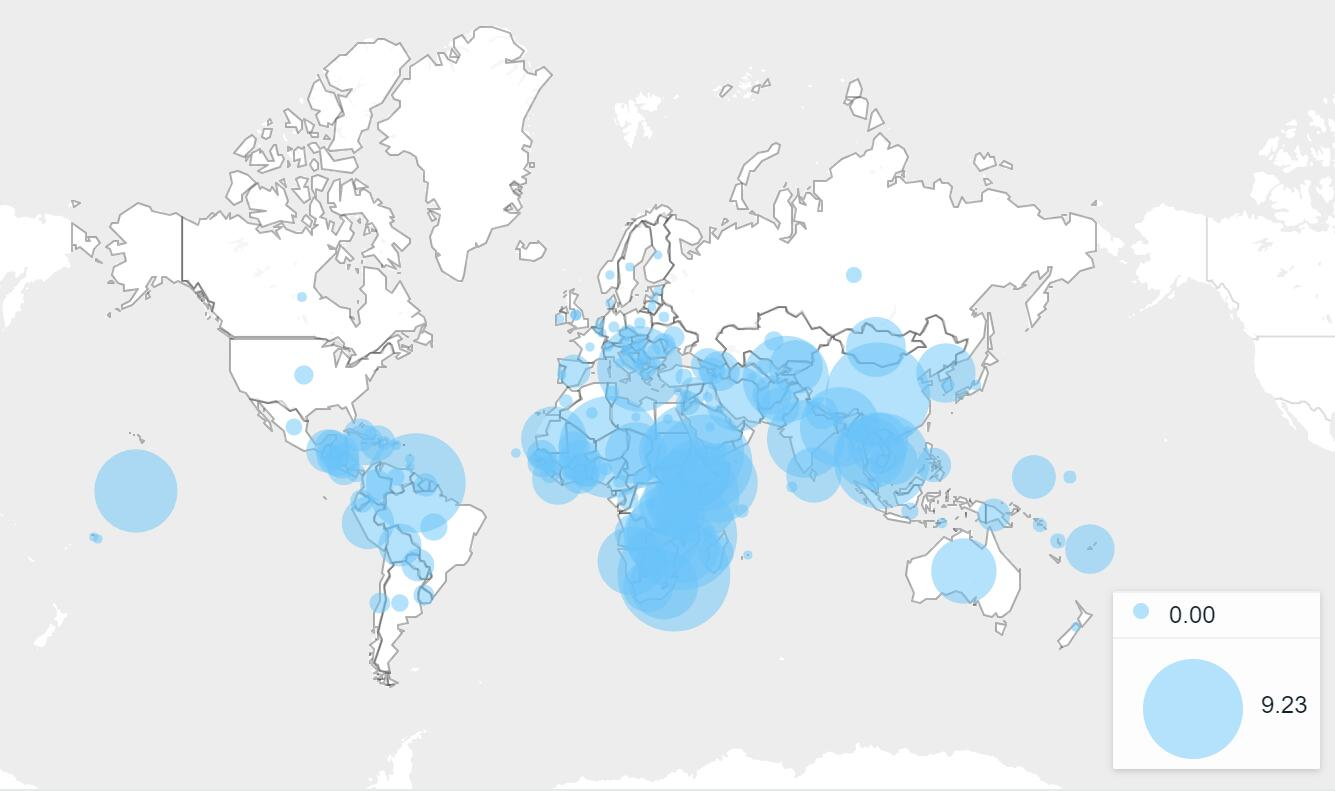
\includegraphics[width=7cm]{weather.jpg}
  \caption{extrame weather}
  \end{minipage}
  \begin{minipage}[h]{0.48\textwidth}
  \centering
  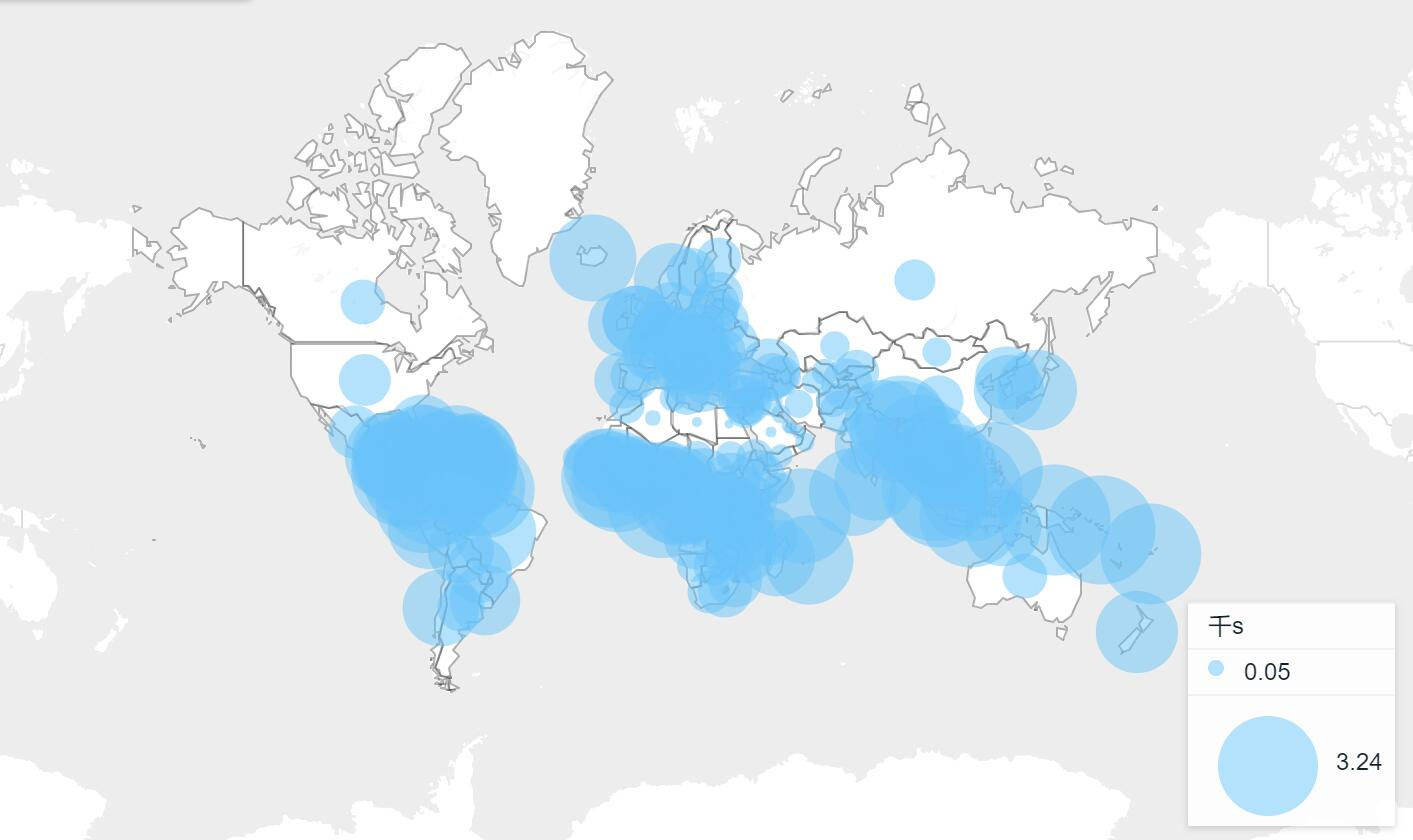
\includegraphics[width=7cm]{rainfall.jpg}
  \caption{water dependency}
  \end{minipage}
\end{figure}
\newpage
It can be seen from the figure that the distribution of the three climatic factors index is basically the same on the map, and more concentrated in Africa, South Asia, which is basically the same as the distribution of the fragility index.
\begin{itemize}
  \item Water dependency ratio refers to a country's dependence on water resources. When climate change has led to a change in the distribution of water resources, regions with larger water dependency ratio tend to exhibit very unoptimistic vulnerabilities. The indicator visually reflects on the map that the darker the color, the larger the value, the stronger its dependence on water resources.
  \item Extreme temperatures index, is the annual average percentage of the population that is affected by natural disasters classified as either droughts, floods, or extreme temperature events. Changes in the climate are often accompanied by extreme weather, making the index larger. This indicator visually reflects on the map as the larger the diameter of the circle, the greater the number of people affected by extreme weather.
  \item The Global Climate Risk Index analyses to what extent countries have been affected by the impacts of weather-related loss events (storms, floods, heat waves etc.) The indicator visually reflects on the map that the darker the color, the larger the value, the more it is affected.
\end{itemize}


\subsubsection{Cohesion Factors}
In general, race and religion are a very important factor affecting the stability of a country. Without effective government control, various kinds of racial and religious affairs in a country mostly lead to instability. The increasing number of refugees in a country can also intensify the complexity of the social situation and put the country on the brink of peril.\\
Comparing the data that we collected with the fragility index given by the subject, we find that in most of the cases, the country with high number of refugees and more varied ethnic and religious diversity has the higher fragility index, such as Africa and Central Asia. So we come to the conclude that this part of the data is valid.\\
\begin{figure}[h]
  \centering
  \begin{minipage}[h]{0.48\textwidth}
  \centering
  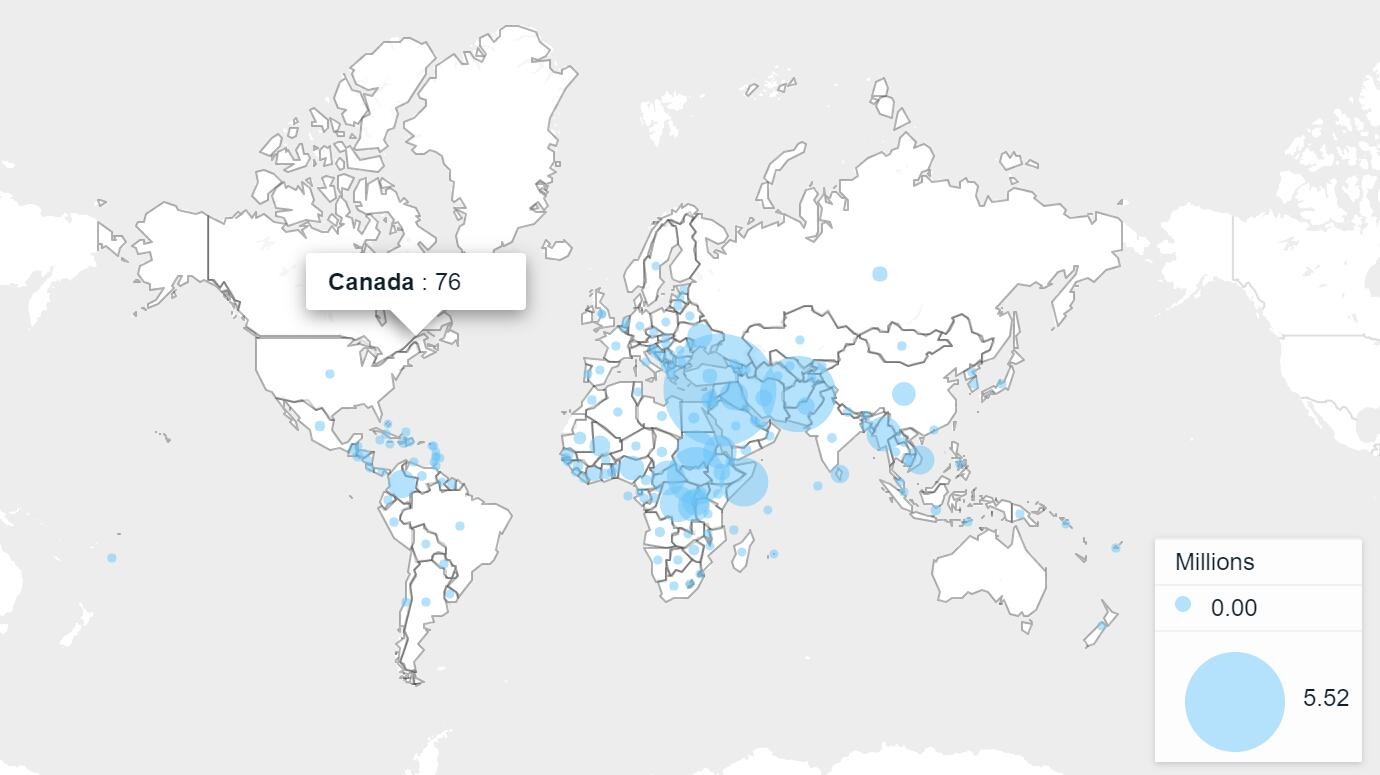
\includegraphics[width=7cm]{refugee.jpg}
  \caption{refugee people number}
  \end{minipage}
  \begin{minipage}[h]{0.48\textwidth}
  \centering
  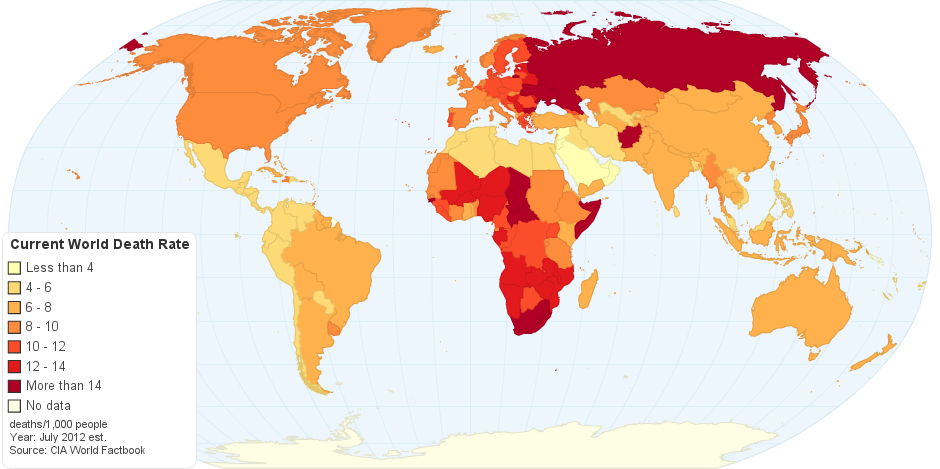
\includegraphics[width=7cm]{death-rate.png}
  \caption{death rate}
  \end{minipage}
\end{figure}
\newpage
It can be seen from the figure that the distribution of the two cohesion factor indices basically coincides with each other on the map forming overlapping parts and is mostly concentrated in Africa, Central Asia and other regions, which is basically the same as that of the fragility index.
\begin{itemize}
  \item One country's refugees are people whose residence are in this country but lose their homes and means of livelihood. The indicator reflects intuitively on a map as a dot. The larger the size, the greater the number of refugees.
  \item Ethnic and cultural diversity index is the quality of diverse or different cultures and ethnicity. The indicator visually reflects on the map that the darker the color, the greater the religious and ethnic diversity.
\end{itemize}


\subsubsection{Economic Factors}
The economic foundation determines the superstructure. An economically underdeveloped country must be a backward country. The higher the share of agriculture in the GDP of a country, the greater the impact on the country from climate change.
Comparing the data we collected with the fragility index given by the subject, we find that the country with higher fragility index, in most of the cases, is in poor economic conditions and has the large share of agriculture in the GDP.  So we can conclude that this part of the data is valid.\\
The figure shows that the distribution of the three economic factors basically displays as coincidence on the map and is mostly concentrated in Africa, which is basically the same as that of the fragility index.
\begin{figure}[h]
  \centering
  \begin{minipage}[h]{0.48\textwidth}
  \centering
  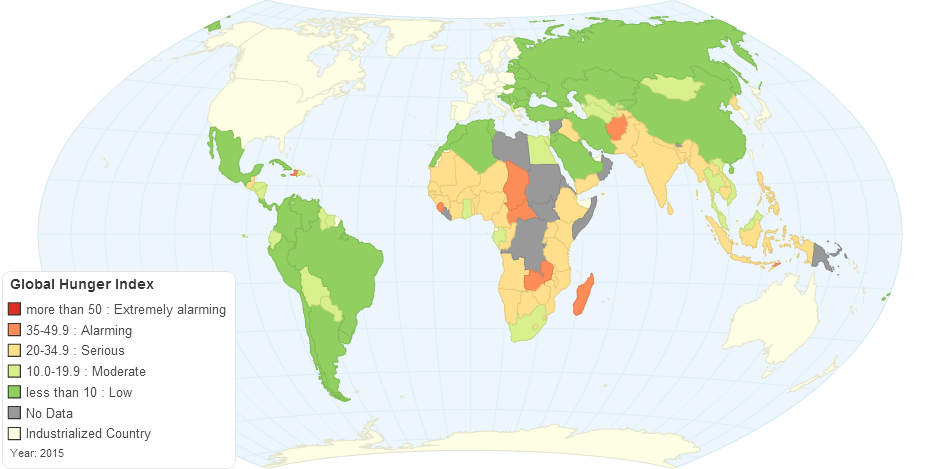
\includegraphics[width=7cm]{hunger.png}
  \caption{global hunger index}
  \end{minipage}
  \begin{minipage}[h]{0.48\textwidth}
  \centering
  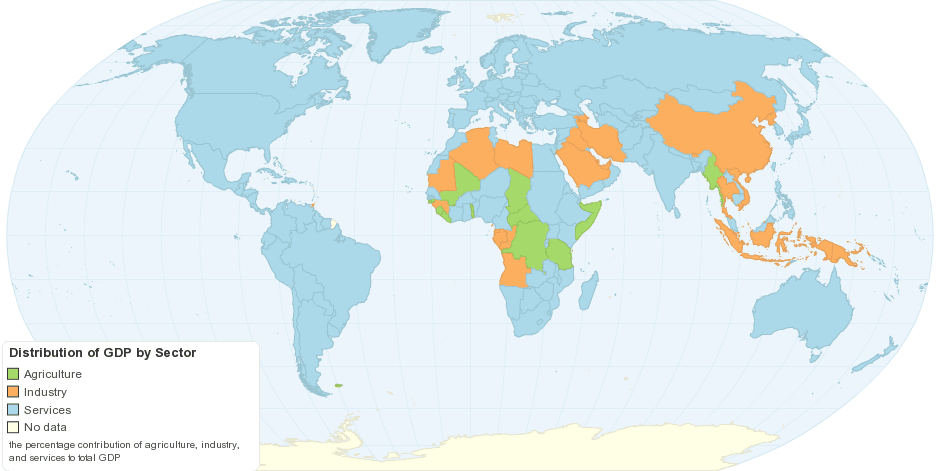
\includegraphics[width=7cm]{agriGDP.png}
  \caption{proportion of agricultural output in GDP}
  \end{minipage}
\end{figure}
\begin{itemize}
  \item GDP per capita is often considered as an indicator of a country's standard of living. The indicator shows visually on the map that the darker the color, the higher the index.
  \item The Global Hunger Index (GHI) is a tool adapted and further developed by the International Food Policy Research Institute (IFPRI) to comprehensively measure and track global hunger. Each color in this figure corresponds to a certain value. The larger the value is, the more people in hungry the country has.
  \item The dependence of the national economy on climate depends on the proportion of agricultural output in GDP. The colors in the figure correspond to the corresponding values, the larger the value is, the stronger the dependence.
\end{itemize}

\subsubsection{Political Facators}
A strong government often can effectively deal with various external factors that may interfere with the stability of the country. Government effectiveness is an important indicator of national fragility. At the same time, the situation in the region is also a very important factor.\\
Comparing the data we collected with the fragility index given by the subject, we find that in most of the cases, countries with poor economic conditions and the proportion of agriculture in GDP is high, the fragility index is also higher. So we can conclude that this part of the data is valid.\\
\begin{figure}[h]
  \centering
  \begin{minipage}[h]{0.48\textwidth}
  \centering
  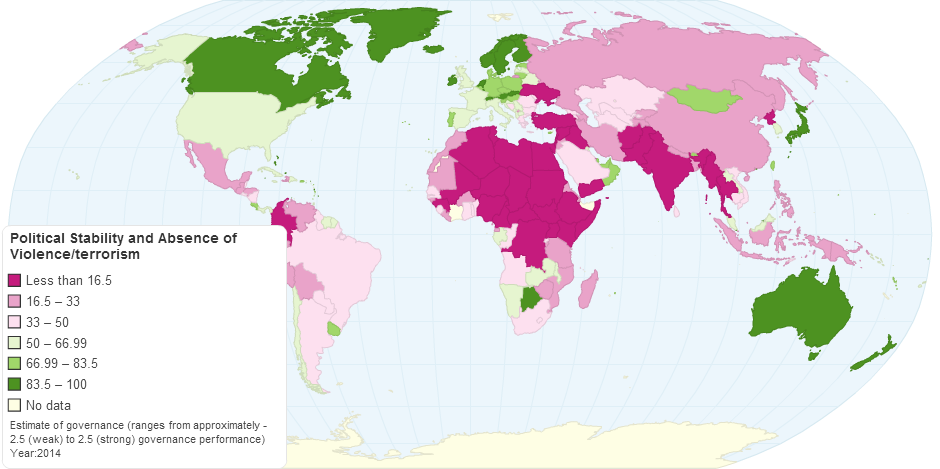
\includegraphics[width=7cm]{govsta.png}
  \caption{political stability index}
  \end{minipage}
  \begin{minipage}[h]{0.48\textwidth}
  \centering
  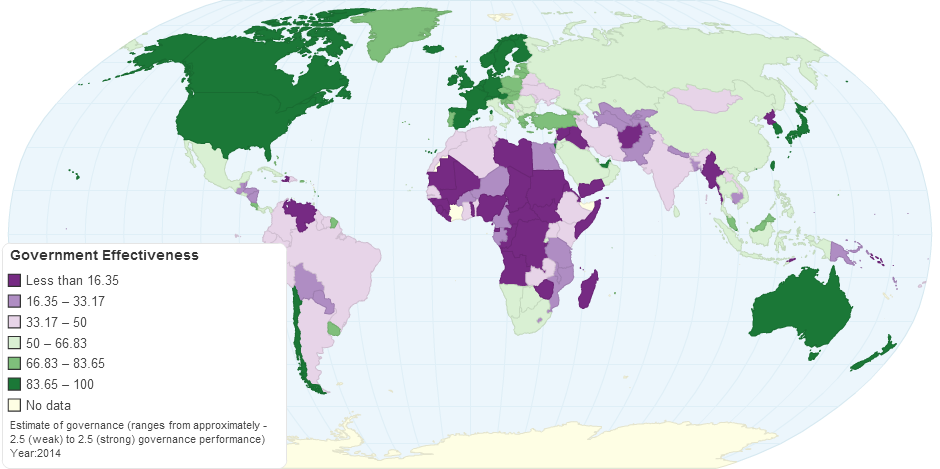
\includegraphics[width=7cm]{govef.png}
  \caption{government effectiveness index}
  \end{minipage}
\end{figure}\\
It can be seen from the figure that the distribution of the strength of the three political factors index basically coincide on the map and are mostly concentrated in the African. This is basically the same as the distribution of fragility. Government effectiveness index reflects perceptions of the quality of public services, the quality of the civil service and the degree of its independence from the political pressures. The colors in the figure correspond to the corresponding values. The lower the values, the worse the government’s effectiveness.
\begin{itemize}
  \item Government effectiveness index reflects perceptions of the quality of public services, the quality of the civil service and the degree of its independence from the political pressures. The colors in the figure correspond to the corresponding values. The lower the values, the worse the government’s effectiveness.
  \item People's freedom index, measures the degree of civil liberties and political rights in every nation and significant related and disputed territories around the world. The colors in the figure corresponds to the corresponding values. The lower the value, the lower the freedom index of citizens.
  \item Political stability index reflects perceptions of the likelihood that the government will be destabilized or overthrown by unconstitutional or violent means. The colors in the figure correspond to corresponding values. The lower the value, the worse the political stability.
  \item Firepower index is based strictly on each nation's potential conventional war-making capability across land, sea and air. The color in the figure corresponds to the corresponding values. The larger the values,the war is more likely.
\end{itemize}

\subsubsection{Socical Factors}
We choose four indices including death rate, crime index, food security index and basic health services index as social factors measuring country fragility, crime index can measure the situation of a country's social stability. Food security index and basic health services index is related to physical condition of national citizens, death rate can measure the living situation of national citizens.\\
While comparing the data we collected with the fragility index given by the topic, we can see, in most condition, the poorer the economy condition is the higher the country fragility index is, meanwhile, the higher the proportion agriculture occupies in GDP, the higher the index is. Thus, we can conclude these data as valid.
\begin{figure}[h]
  \centering
  \begin{minipage}[h]{0.48\textwidth}
  \centering
  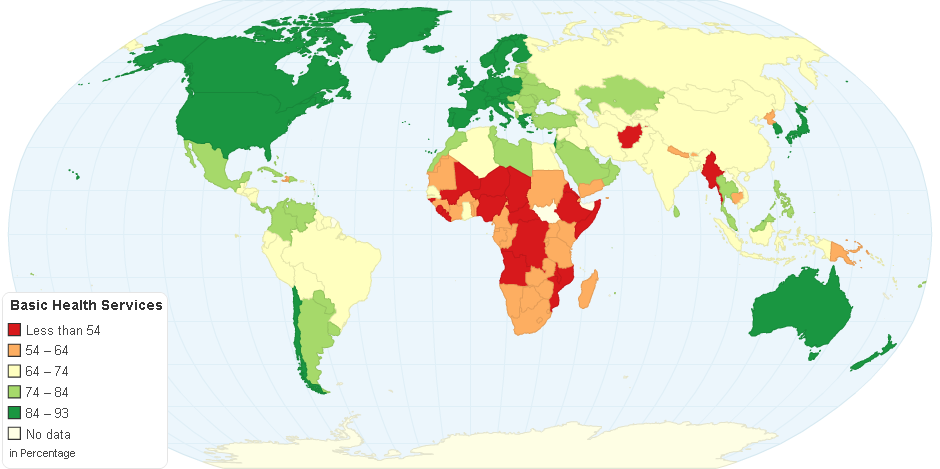
\includegraphics[width=7cm]{sanitation.png}
  \caption{basic health services index}
  \end{minipage}
  \begin{minipage}[h]{0.48\textwidth}
  \centering
  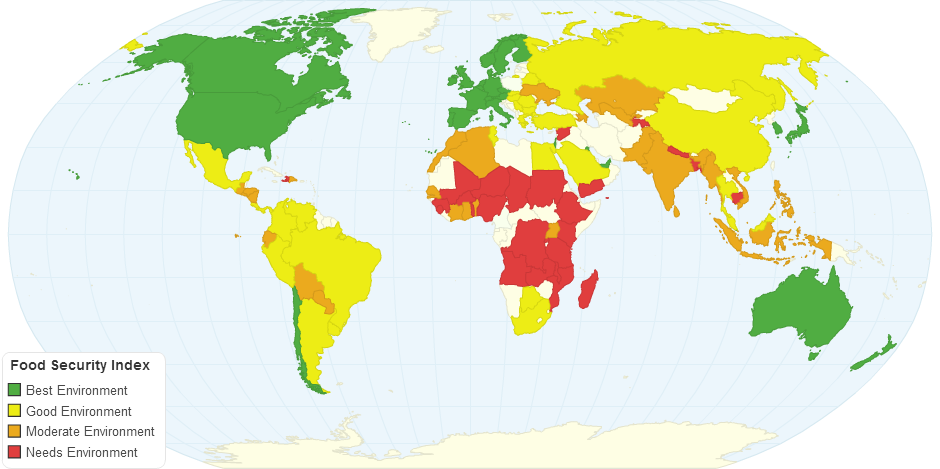
\includegraphics[width=7cm]{food.png}
  \caption{food security index}
  \end{minipage}
\end{figure}
As we can see in the map, the degree of these three social factors is basically coincident, mainly aggregate in Africa, which is basically the same as the distribution of fragility index.
\begin{itemize}
  \item Crime index is an evaluation of criminal frequency in a country, the colors in the map correspond to different value, the higher the value, the higher the seriousness of crime is.
  \item Food security index, provides a worldwide perspective on which countries are the most and least vulnerable to food insecurity. The colors in the map correspond to different value. The higher the value is, the higher the degree of food security is.
  \item Basic health services index reflects the degree of dissemination of health services in a country, the higher the value is, the higher the degree of health service dissemination is.
  \item Death rate compares the average annual number of deaths during a year per 1,000 population at midyear, reflects the social stability of a country indirectly, the colors in the map correspond to different value. The higher the value is, the higher the death rate is.
\end{itemize}
\newpage
\section{Variable Description}
% 表格
\begin{table}[h]
  \linespread{1.0}
  \centering
  \caption{Variables}
  \label{my-label}
  \setlength{\tabcolsep}{7mm}{
  \begin{tabular}{l|l|l|l|l|l|l|l|l|l|l|l}
  \shline
  \multicolumn{2}{lI}{\textbf{variable}} & \multicolumn{10}{l}{\textbf{description}} \\ \hline
  \multicolumn{2}{lI}{GDP}           & \multicolumn{10}{l}{Gross Domestic Product per capita}    \\ \hline
  \multicolumn{2}{lI}{REF}           & \multicolumn{10}{l}{refugee people number}               \\ \hline
  \multicolumn{2}{lI}{WDR}           & \multicolumn{10}{l}{water dependency ratio}            \\ \hline
  \multicolumn{2}{lI}{ETI}           & \multicolumn{10}{l}{extreme temperatures index}         \\ \hline
  \multicolumn{2}{lI}{NDI}           & \multicolumn{10}{l}{natural disaster index}             \\ \hline
  \multicolumn{2}{lI}{ECD}           & \multicolumn{10}{l}{ethnic and cultural diversity index}        \\ \hline
  \multicolumn{2}{lI}{HUG}           & \multicolumn{10}{l}{global hunger index}                                \\ \hline
  \multicolumn{2}{lI}{AGR}           & \multicolumn{10}{l}{proportion of agricultural output in GDP}              \\ \hline
  \multicolumn{2}{lI}{GEF}           & \multicolumn{10}{l}{government effectiveness index}              \\ \hline
  \multicolumn{2}{lI}{FRE}           & \multicolumn{10}{l}{poeple's fredom index}              \\ \hline
  \multicolumn{2}{lI}{STA}           & \multicolumn{10}{l}{political stability index}              \\ \hline
  \multicolumn{2}{lI}{FIP}           & \multicolumn{10}{l}{global firepower index}              \\ \hline
  \multicolumn{2}{lI}{DEA}           & \multicolumn{10}{l}{death rate}              \\ \hline
  \multicolumn{2}{lI}{CRI}           & \multicolumn{10}{l}{crime index}              \\ \hline
  \multicolumn{2}{lI}{FDS}           & \multicolumn{10}{l}{food security index}              \\ \hline
  \multicolumn{2}{lI}{BHS}           & \multicolumn{10}{l}{basic health services index}              \\ \shline
  \end{tabular}}
  \end{table}  
% 插图
% \begin{figure}[h]
% \small
% \centering
% 
\includegraphics[width=12cm]{test1.jpg}
% \caption{asssssa} \label{fig:aa}
% \end{figure}

% 引用
% \eqref{aa}
% \begin{equation}
% a^2 \label{aa}
% \end{equation}

% 公式
% \[
%   \frac{\mathrm{d} C_{1}}{\mathrm{d} t}= \left 
%   ( 1-\frac{C}{R} \right )^{P_{I}}\frac{\mathrm{d} I}
%   {\mathrm{d} t}\frac{C_{I}}{I} \eqno (3)
% \]




\section{Fragile State Neural Network Model}
The study of national fragility indicators requires strong professional
background knowledge, but we can't derive the relationship between climate
and fragility through an intuitive approach from the data given in the 
problem. So, through collecting data, by using the strong self-organization, 
self-adaptive and self-learning ability of neural network, the nonlinear 
mapping of independent variables and national fragility can be completed 
without fully understanding the relationship among climate, politics, 
economy and national fragility. Combined with the above considerations, 
We established a neural network to derive a national fragility model 
including climatic factors.
\subsection{Model building}
\subsubsection{Introduction to the principle of BP Neural Network}
BP Neural Network is a kind of multi-layer feedforward neural network, 
which is mainly characterized by forward transmission and deviation back 
propagation. In forward transmission, the input signal is processed from 
the input layer through the hidden layer to the output layer. The state of 
each layer of neurons affects only the next layer of neurons. If the output 
layer does not get the desired output, it is transferred to the reverse 
propagation, and the network weight and threshold are adjusted according 
to the predicted error, so that the BP Neural Network prediction output 
is constantly approaching the expected output. A simple BP Neural Network 
is like Figure \ref{fig:nn} as follow.\upcite{bib20}
\begin{figure}[h]
\small
\centering
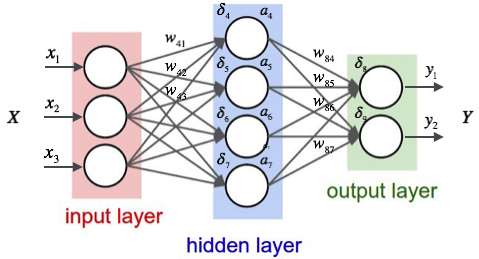
\includegraphics[width=10cm]{neuralNetwork.png}
\caption{a BP Neural Network} 
\label{fig:nn}
\end{figure}

\newpage
\subsubsection{Data preprocessing}
Based on our hypothesis, the fragility of a country is related to its 
sensitivity and adaptability. Sensitivity and adaptability are closely 
related to economic conditions, political conditions, social conditions and 
climate change, and can be quantified with a numerical value. The sensitivity 
may be composed of extreme weather, the average depth of precipitation, the 
climate sensitivity index, the index of food security, the country risk index, 
the index of health, mortality, crime, global power index, hunger, agricultural 
development index, the number of ethnic diversity and refugees. Due to a variety 
of data among different indicators, some data are often hundreds of thousands of, 
and some data is within the scope of a single wave, so we each data respectively 
for the normalized processing, allow them to operations in the same numerical range, 
convenient for our model. The normalization method is as follows:
\[ y=\frac{\left ( y_{max}-y_{min} \right )\left ( x-x_{min} \right )}{x_{max}-x_{min}}+y_{min} \]
With the formula above, we can begin to build our model after the data we have 
collected is normalized. This can be done by calling the transform() function 
of sklearn. 
\subsubsection{Establish BP Neural Network}
We used Google's machine learning framework, TensorFlow, to establish the BP 
Neural Network structure of x-n-2, where X represents the input item (that is, 
the data mentioned in the data analysis); N is the number of hidden layer neurons; 2 
represents the output item (sensitivity and adaptability). The structure diagram is 
as follows:
\begin{figure}[h]
\small
\centering
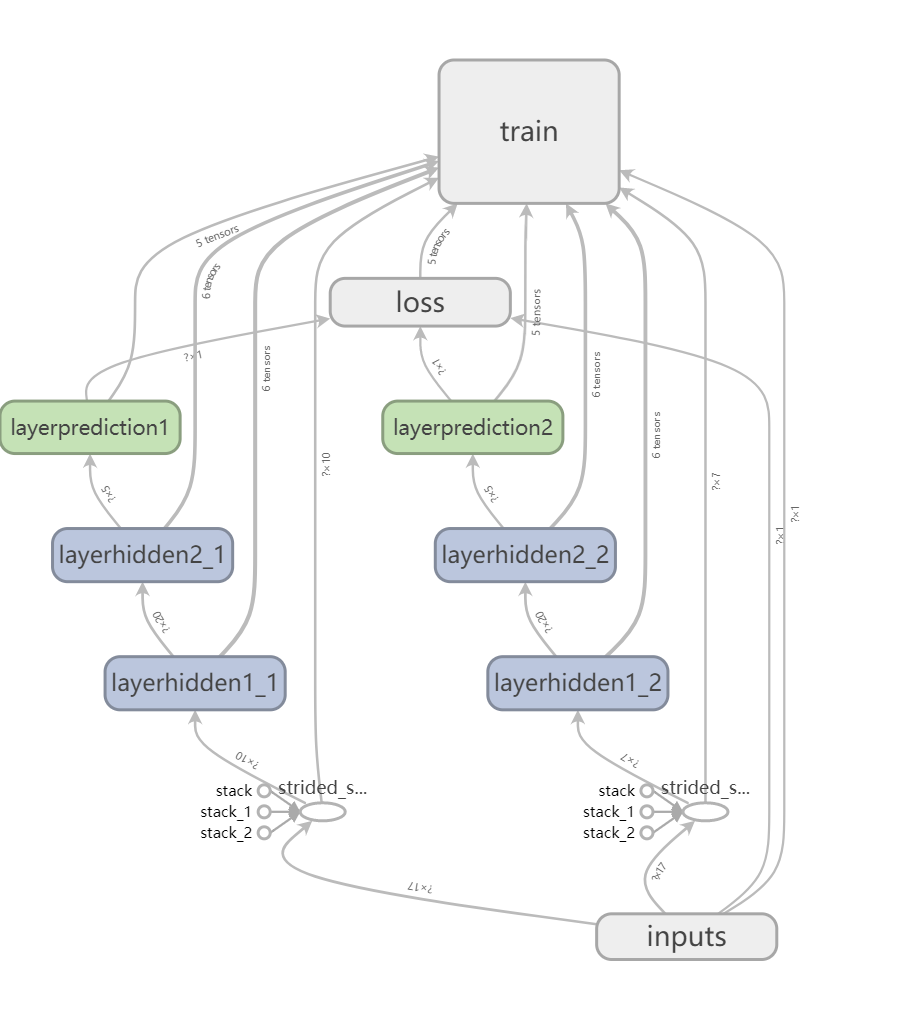
\includegraphics[width=10cm]{structure.png}
\caption{Network Structure} 
\label{fig:ns}
\end{figure}\\
\newpage
We choose ReLU(Rectified Linear Unit) as hidden layer excitation function:
\[ f=max\left ( 0,w^{T}x+b \right ) \]
And linear function as the output layer Excitation function:
\[ a=n \]
The number of hidden layer neurons has a significant influence on 
the prediction accuracy of BP Neural Network. If the number of 
nodes is too few, the network will not learn well and the accuracy 
will be not enough. If the number of nodes is too many, the 
training time increases, the network is easy to be overfitting. 
We refer to the following formula to determine the optimal number 
of hidden layer neurons.
\[ l< n-1 \]
\[ l<\sqrt{m+n}+a \]
\[ l=\log_{2} n \]
In the formula, n is the input layer node number, L is the hidden 
layer node number, M is the output layer node number, A is the constant 
between the 0~10. In practical problems, the selection of the number 
of hidden layer nodes first uses the reference formula to determine 
the approximate range of the number of nodes, and then the optimal 
node number is determined by the method of trial-and-order. After 
many experiments, we choose n=100, at this time the BP Neural Network 
achieves high precision. Learning speed also has an important influence 
on the BP Neural Network, the learning speed is too small, the 
network learning is slow, need to increase the training times, the 
learning speed is too big, the network learns quickly, but easily 
leads to the network not to converge, affects the training precision. 
We finally decided to study at a speed of 0.01, training times 300. 
BP Neural Network using gradient correction method as weights and 
thresholds of learning algorithm, from the network prediction error 
in the negative gradient direction correction weights and thresholds, 
not to consider the accumulation of previous experience, learning 
process convergence is slow. For this problem, the additional momentum 
method can be used to solve the weighted value learning formula 
with additional momentum:
\[ w\left ( k \right )=
w\left ( k-1 \right )+\Delta w\left 
( k \right )+a\left [ w\left ( k-1 \right )-w\left 
( k-2 \right ) \right ] \]
The model will eventually output two results, one is national 
sensitivity, one is national adaptability, we define:
\[ Fragility = Sensitivity - Adaptability \]
Based on this formula, we are able to obtain the 
fragility of the State through the two values of the model output
\subsection{Model Testing}
We use 70\% of the data set as the training data set, and the rest is used as a test data set. And we use MSE to evaluate the model.
\[MSE=\frac{1}{n}\sum_{n}^{t-1}\left ( observed_{t} -predicted_{t}\right)^{2}\]

We get the loss of the model as follow:\\
\begin{figure}[h]
\small
\centering
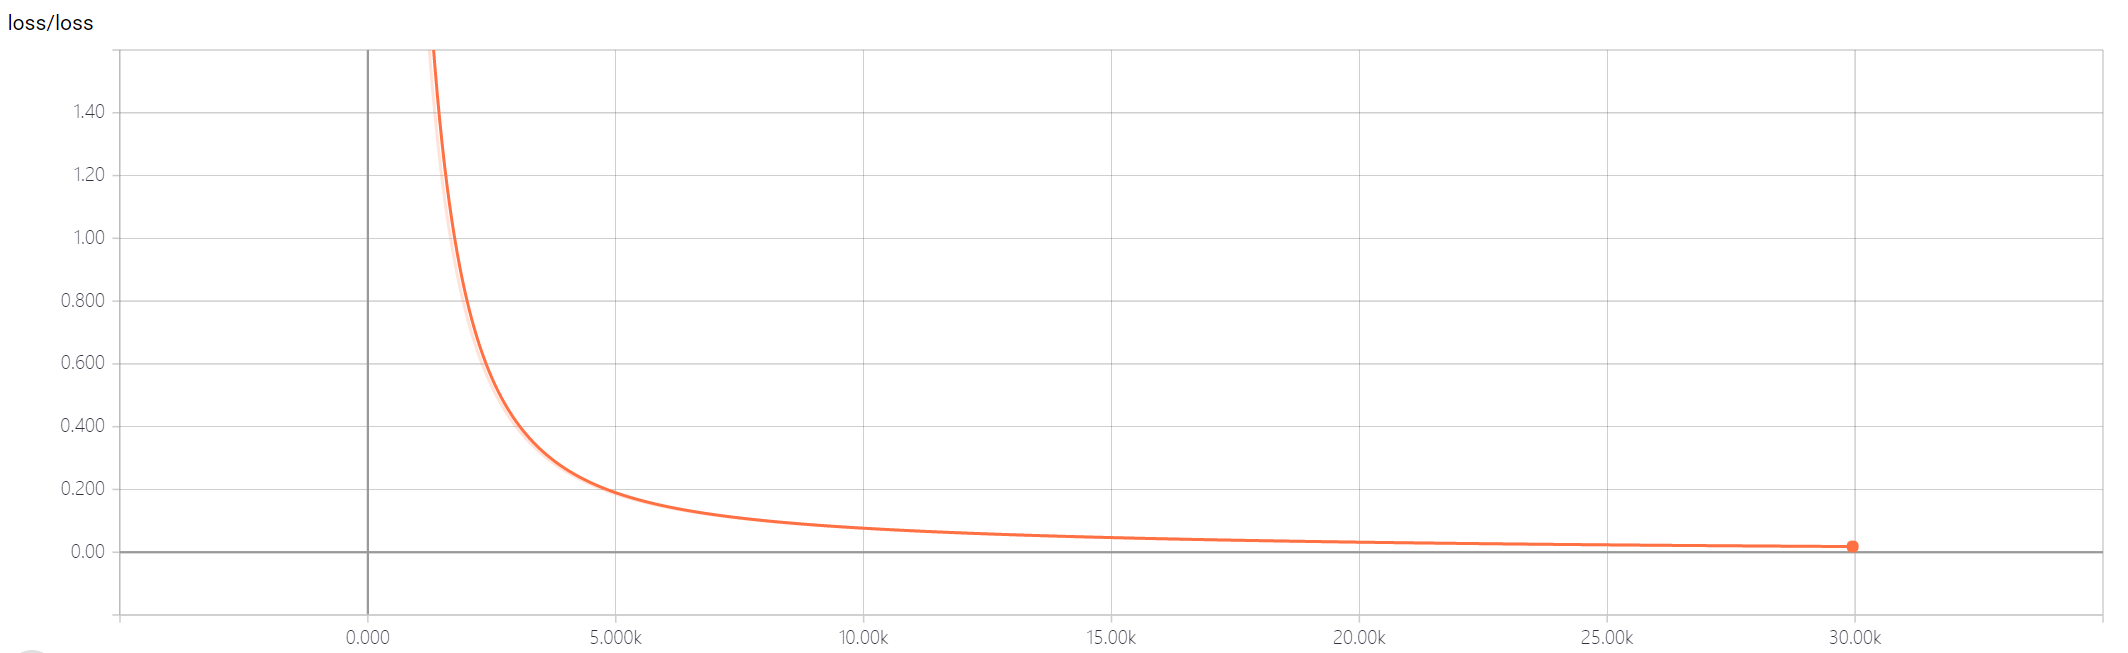
\includegraphics[width=14cm]{loss.png}
\caption{Loss} 
\label{fig:lf}
\end{figure}\\

Finally, MSE converges to 0.12
The model is pretty accurate when the training step is increased to 15.00k.
\subsection{Task I}
According to the output of our model, we divide it into 
three numerical value range referring to the standard in website 
FSI, namely 0-60, 60-90, 90-120. By normalizing them, they 
correspond respectively to the fragile, less fragile, and stable 
state of the country. For our definition, fragility is equal to 
sensibility minus adaptability, so the climatic factor exerts 
influence on the fragility by changing sensibility directly, 
we can present the consequences visually with the line chart 
appointing climate as independent variable, by holding other 
factors constant. 
\begin{figure}[h]
  \centering
  \begin{minipage}[h]{0.3\textwidth}
  \centering
  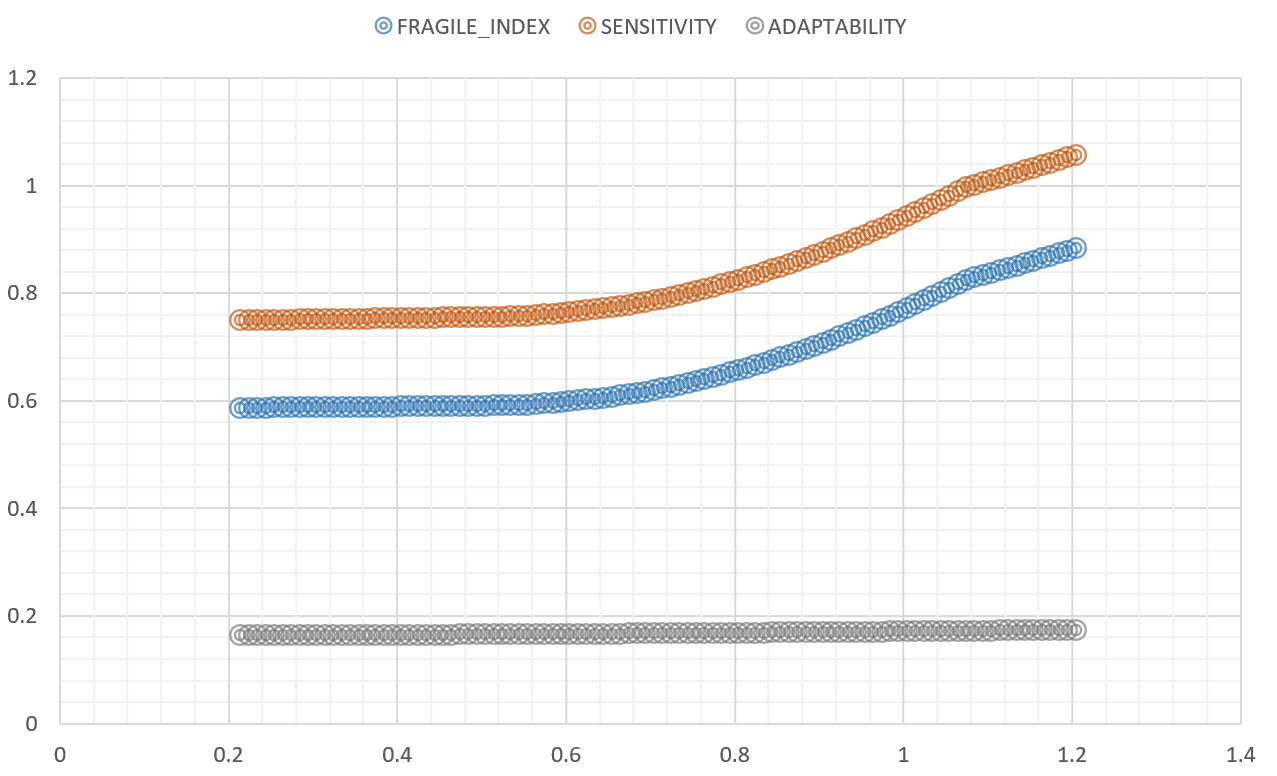
\includegraphics[width=5cm]{task1-1.png}
  \caption{ETI}
  \end{minipage}
  \begin{minipage}[h]{0.3\textwidth}
  \centering
  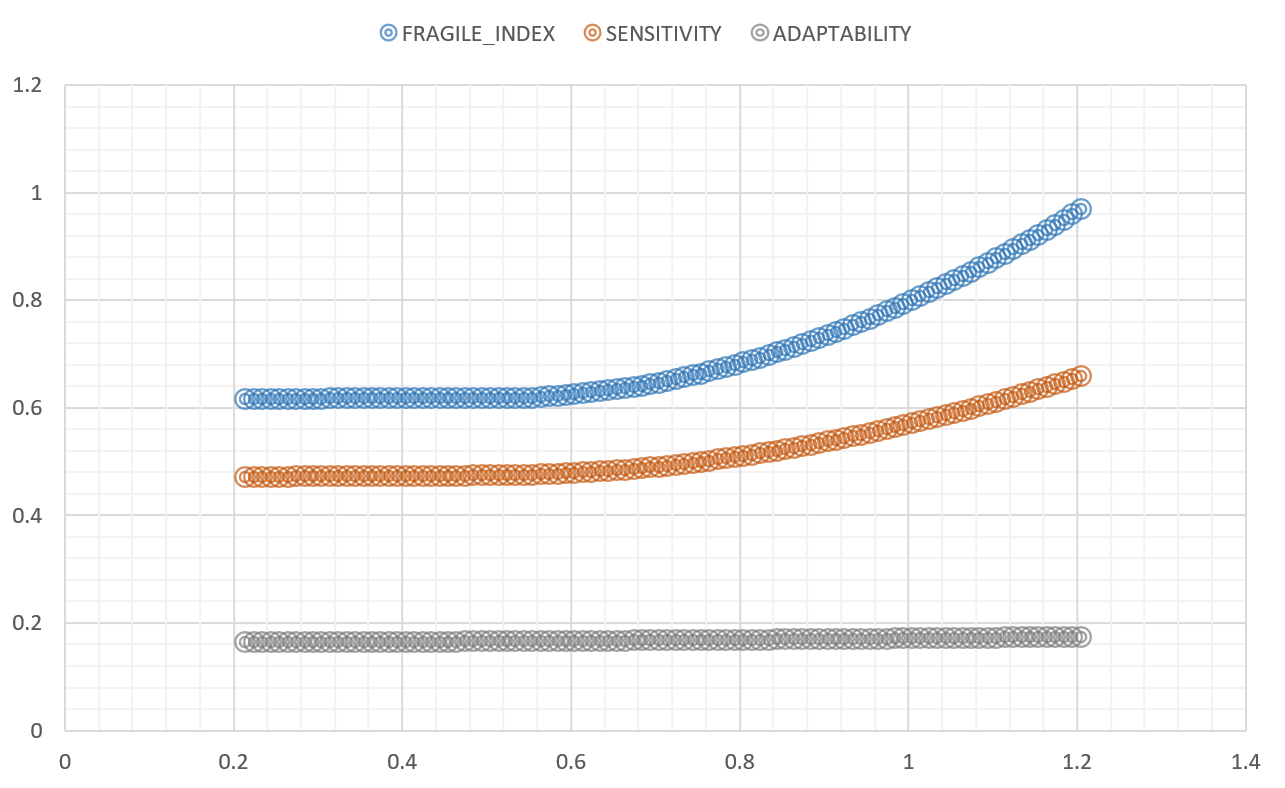
\includegraphics[width=5cm]{task1-2.png}
  \caption{WDR}
  \end{minipage}    
  \begin{minipage}[h]{0.3\textwidth}
  \centering
  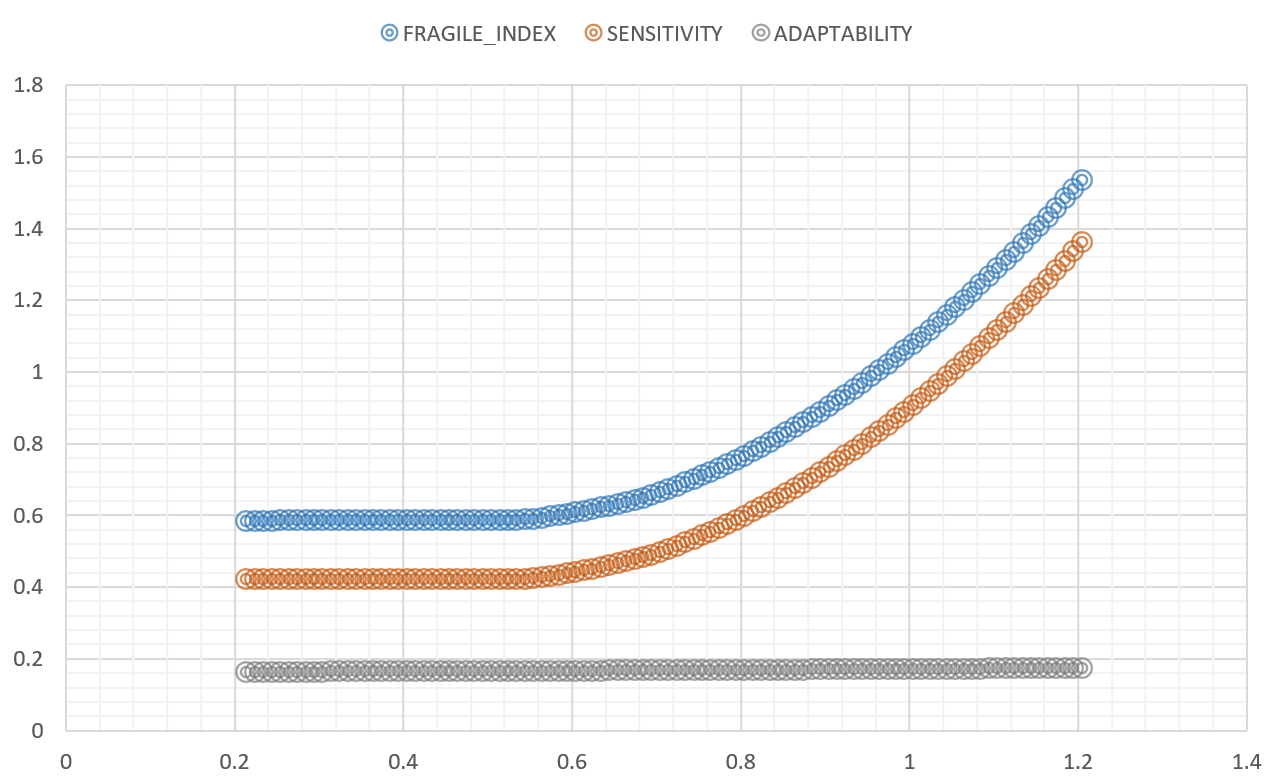
\includegraphics[width=5cm]{task1-3.png}
  \caption{NDI}
  \end{minipage}  
\end{figure}
As for the indirect influence of climate towards 
fragility, firstly, we need to calculate the correlation between 
country sensibility and other factors except for the climate, then 
we pick up factors with strong correlation, after that, we 
calculate the correlation between the climate factors and the 
chosen factors, if the correlation is strong, then we can say 
the climate exerts influence on the country fragility indirectly 
by influencing the chosen factors.
\begin{figure}[h]
  \centering
  \begin{minipage}[h]{0.3\textwidth}
  \centering
  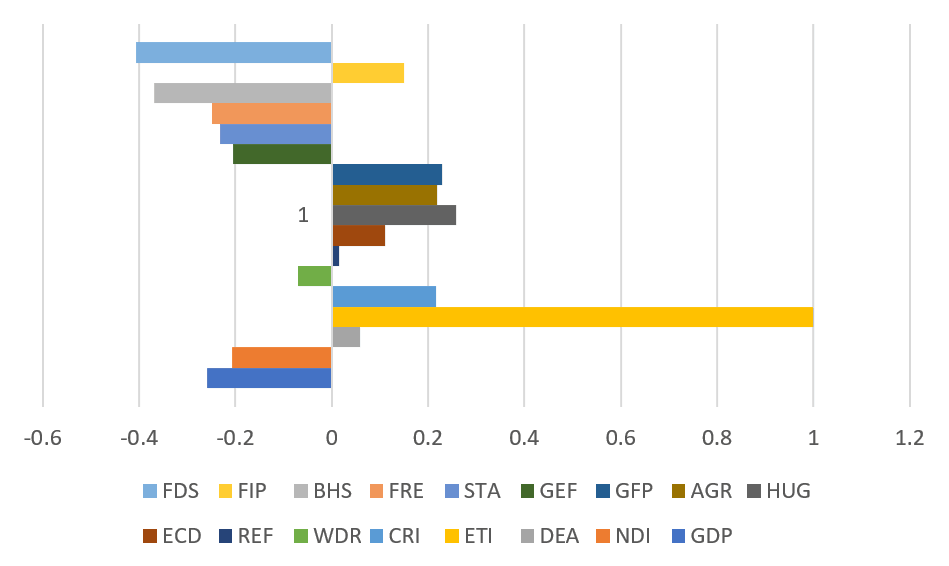
\includegraphics[width=5cm]{task1-4.png}
  \caption{ETI}
  \end{minipage}
  \begin{minipage}[h]{0.3\textwidth}
  \centering
  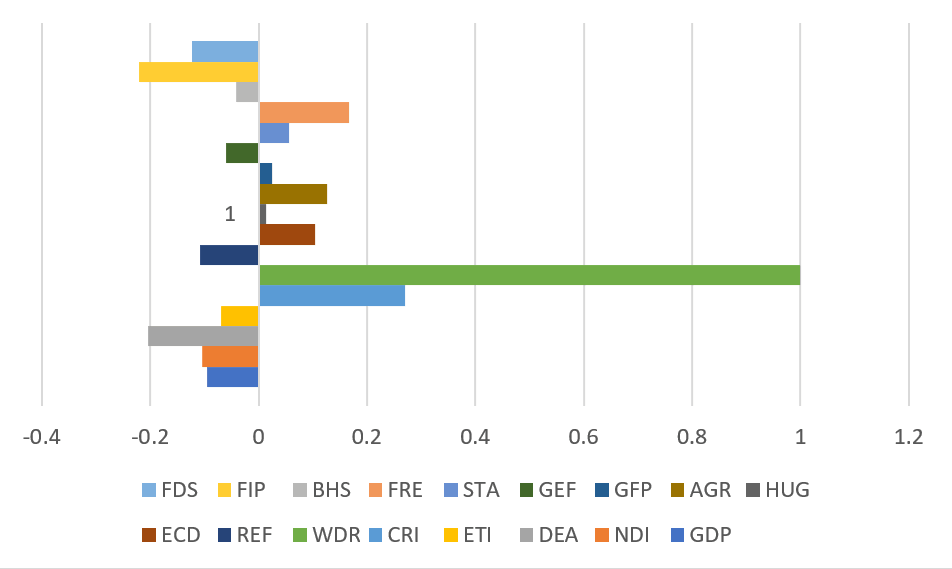
\includegraphics[width=5cm]{task1-5.png}
  \caption{WDR}
  \end{minipage}    
  \begin{minipage}[h]{0.3\textwidth}
  \centering
  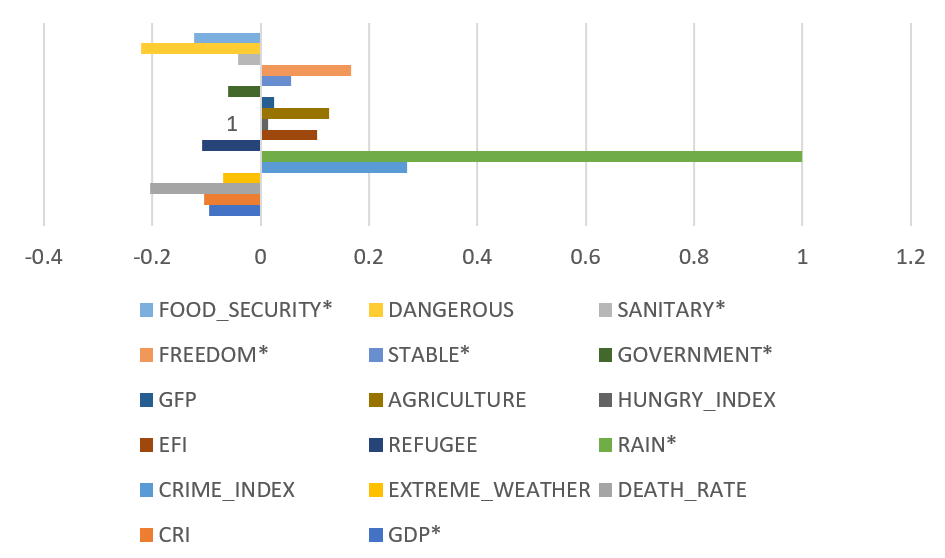
\includegraphics[width=5cm]{task1-6.png}
  \caption{NDI}
  \end{minipage}  
\end{figure}\\
From the charts, we can see the climate mainly exerts 
an effect on the crime index, hungry index, agriculture of 
a country, firepower index, then increases the 
country fragility.
% \newpage
\subsection{Task II}
We choose Sultan in the ten most fragile countries given by FSI , 
to investigate the influence that the climate exerts on the country fragility, 
we need to hold other factors constant, because of the constant factors, 
we can assume the country adaptability constant, the factors that influence 
its fragility are variation of its sensibility due to the climate change, 
change the relevant factors of climate, we get the charts below to show 
how the climate affects its sensibility, and then fragility.
% 这是task2的三张图
\begin{figure}[h]
  \begin{minipage}[h]{0.48\textwidth}
  \flushleft
  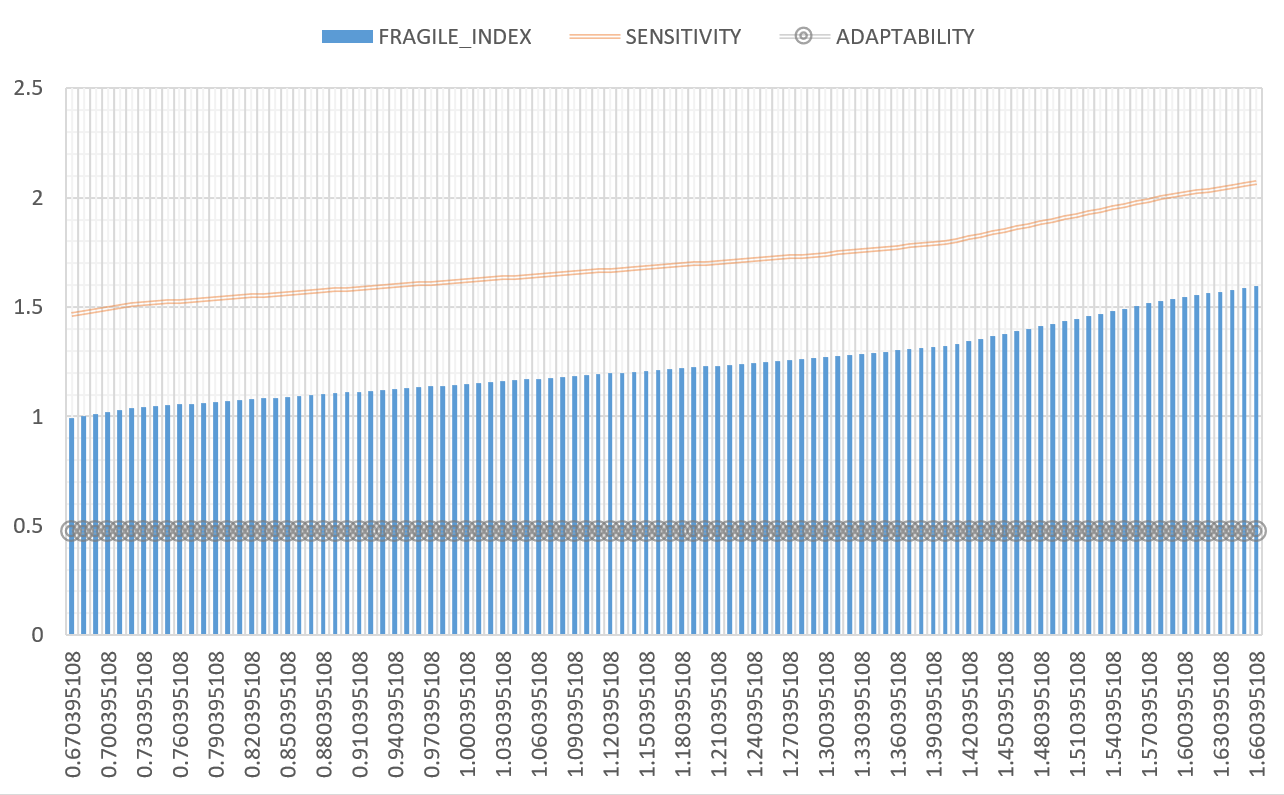
\includegraphics[width=8cm]{task2Weather.png}
  \caption{extrame weather}
  \end{minipage}
  \begin{minipage}[h]{0.48\textwidth}
  \flushright
  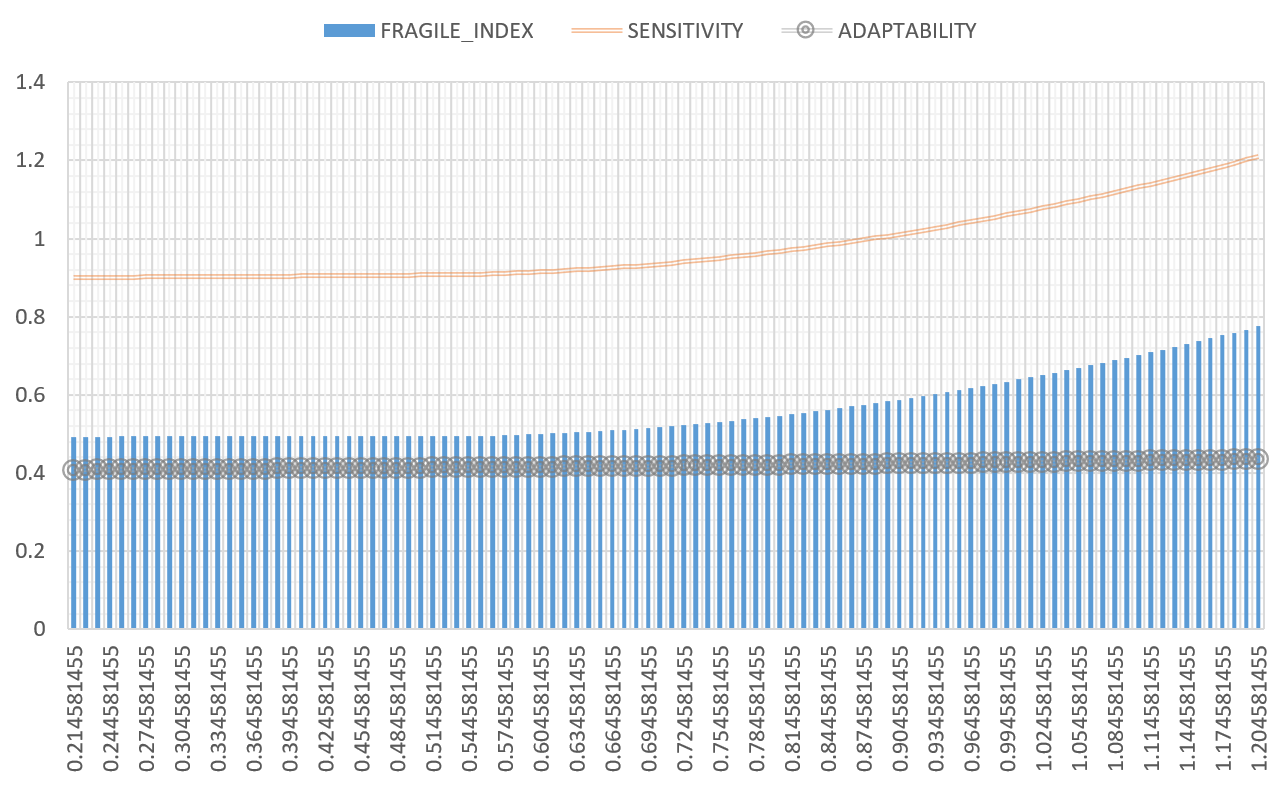
\includegraphics[width=8cm]{task2CRI.png}
  \caption{CRI}
  \end{minipage} 
\end{figure}
% 以上是前两张,这是最后一张
\begin{figure}[h]
  \begin{minipage}[h]{0.50\textwidth}
  \flushleft
  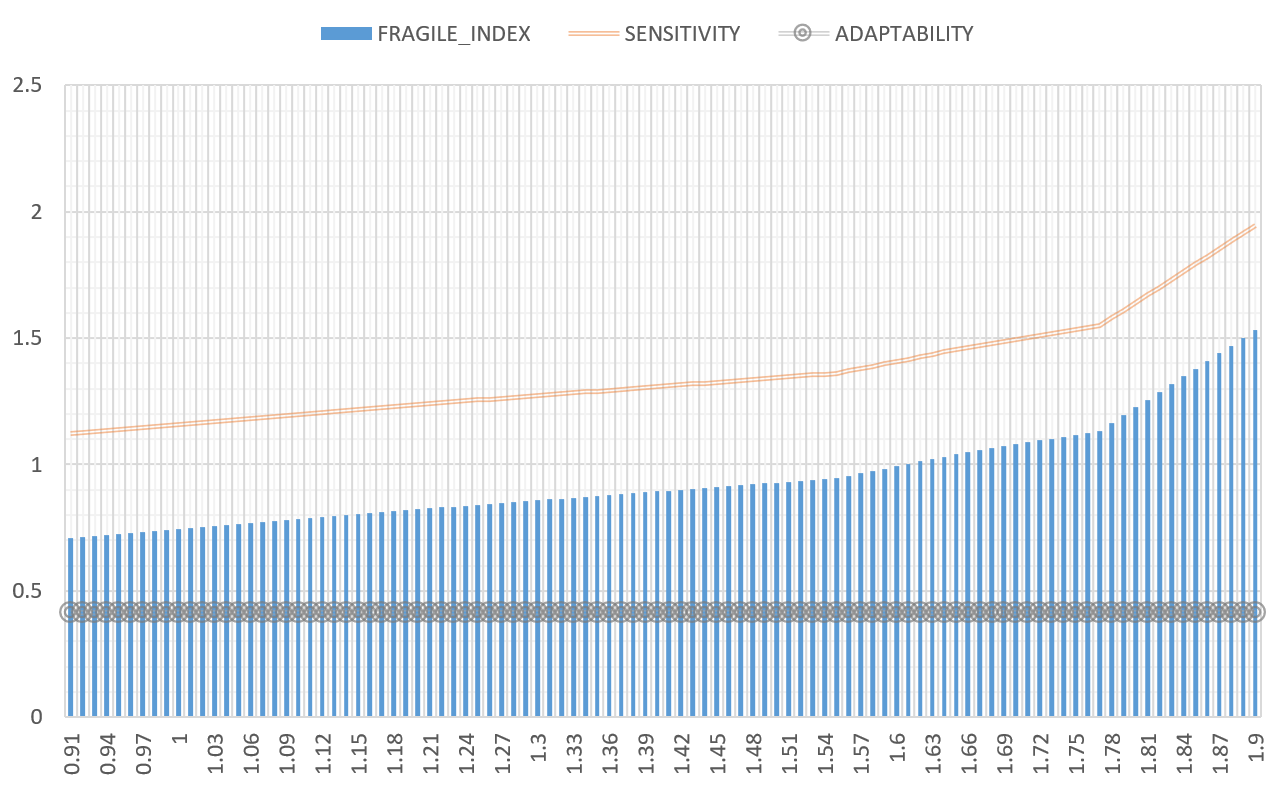
\includegraphics[width=8cm]{task2Rain.png}
  \caption{water dependency ratio}
  \end{minipage}
\end{figure} \\
From the graph we can see the impact of three climatic factors on fragility, 
the impact of natural disaster indices and water resource dependency on fragility, 
and if both are reduced, the fragility of the State can be significantly reduced.
\newpage
\subsection{Task III}
We select Turkey out of the 10 most vulnerable countries in the data given by FSI. To examine how the climate affects fragility, we assume that climatic factors are determined only by extreme weather, water dependence ratio, and natural disaster index.\\
We take these three factors as independent variables to establish three-dimensional coordinate system, and a divide each factors into five levels according to different numerical range,and take the median of each level range as the value of this level input to the model. That is to say, we only need to input a three-dimensional coordinate that we can get the fragility output.\\
Because the coordinate system is three-dimensional, we classify the degree of fragility by finding the isosurface of a particular value. We define isosurface which is equal to 90 (normalized to 0.75) divides  "fragility" and "less fragile", the isosurface which is equal to 60 (normalized to 0.43) divides "less fragile" and "stable".
\begin{figure}[h]
  \begin{minipage}[h]{0.48\textwidth}
  \flushleft
  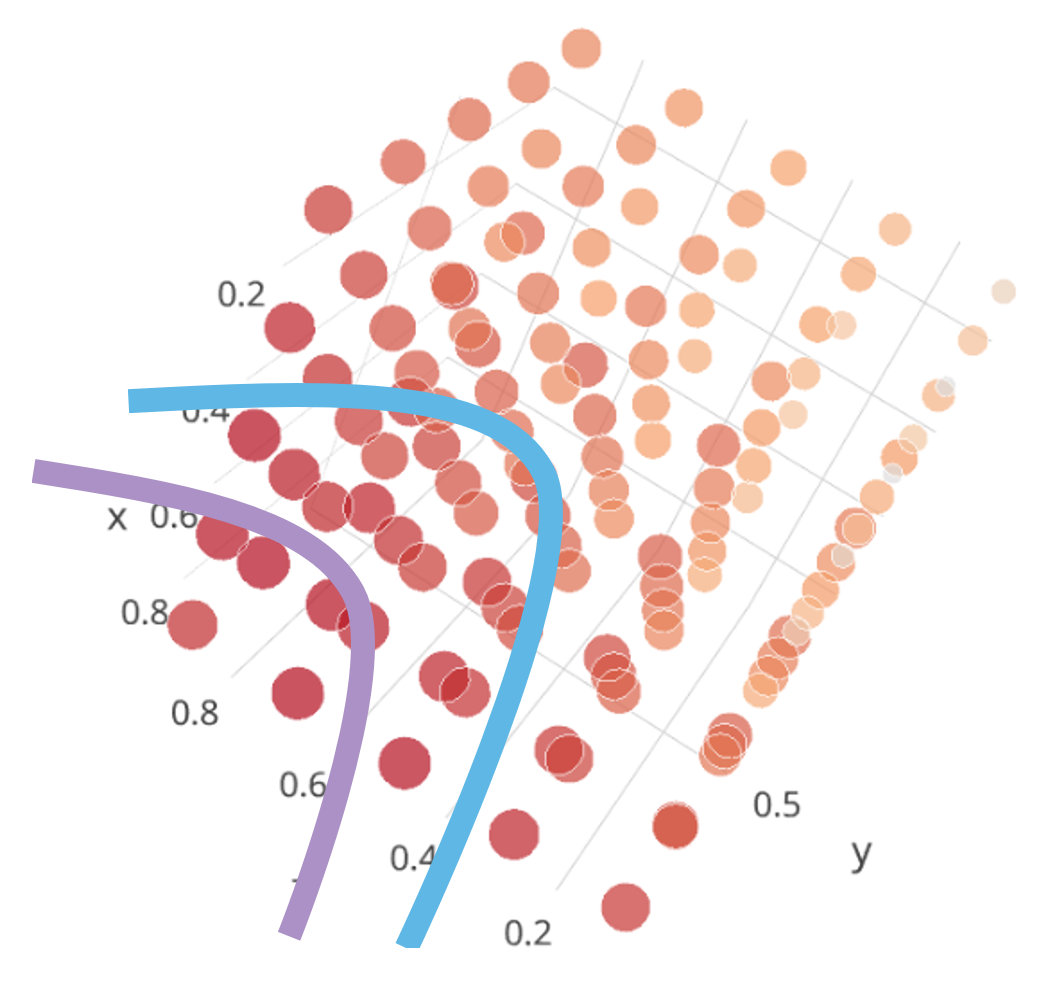
\includegraphics[width=8cm]{task3-1.png}
  \caption{3D scatter point graph}
  \end{minipage}
  \begin{minipage}[h]{0.48\textwidth}
  \flushright
  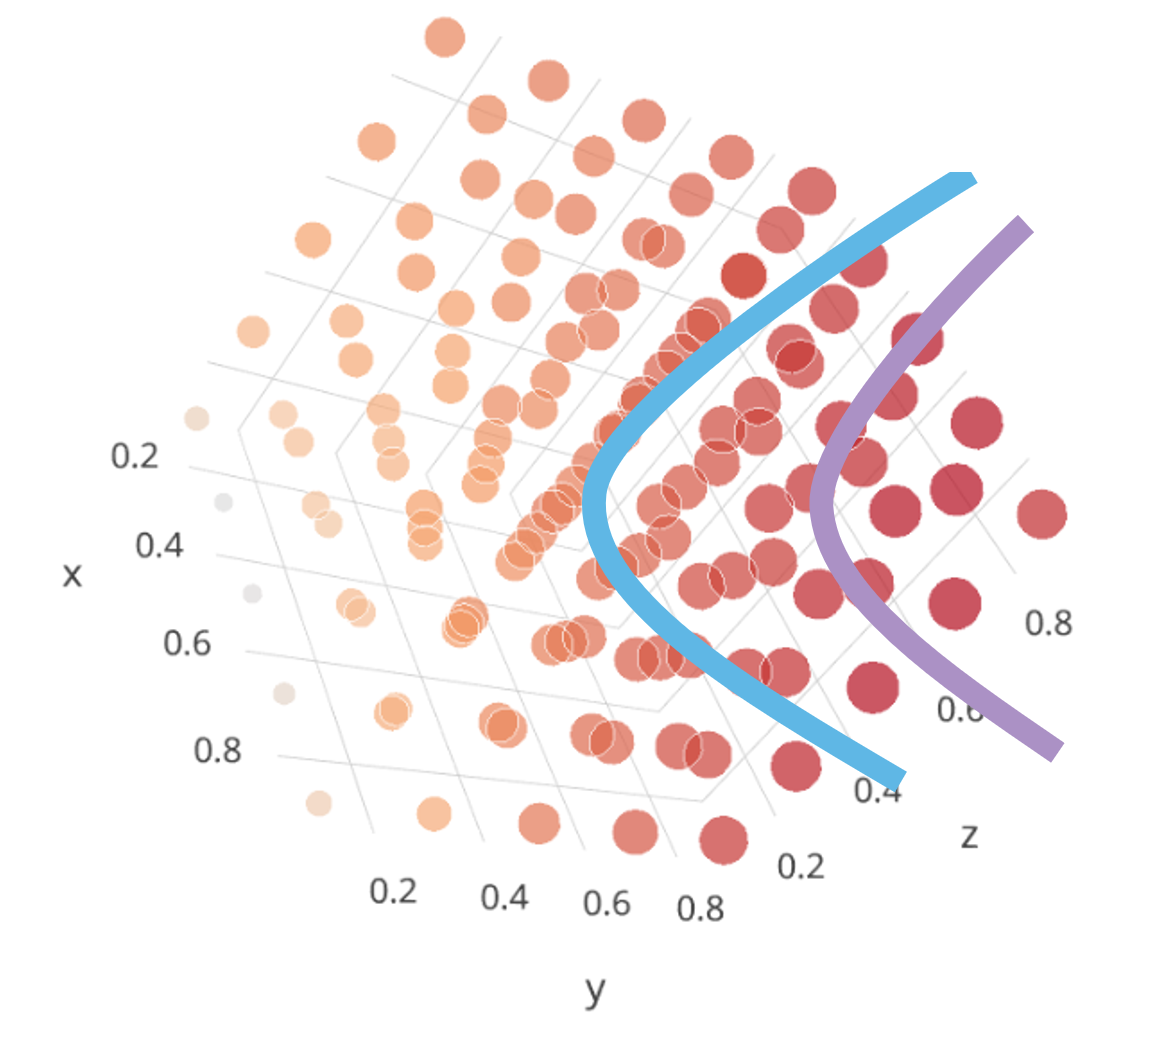
\includegraphics[width=8cm]{task3-2.png}
  \caption{3D scatter point graph}
  \end{minipage}
\end{figure} \\
\newpage
In the graph, x represents WDI, y represents NDI, z represents ETI. 
If we need a more precise interface, we can do this by dividing these factors into more levels. By continually dividing more levels, the value of each factor becomes more accurate, so that we can find a more accurate critical surface.
\subsection{Task IV}
According to the formula we gave earlier:
\textbf{Fragility = Sensitivity - Adaptability}, 
because sensitivity is mainly determined by some non-state 
factors, the impact of state intervention on fragility 
is mainly achieved by changing the country's adaptability. 
According to our hypothesis, the adaptability of the country 
is only determined by GDP per capita, Health index, civil 
rights index, government energy efficiency index, government 
stability index and food safety index. Therefore, we can 
determine how to conduct national intervention by observing 
the output value of our BP Neural Network model and changing 
the above parameters that affect national adaptability, to be 
more likely to prevent the country from becoming a vulnerable 
one. As an example, the following is the relationship between 
sanitation index and adaptability, and the change in fragility 
also manifests.
\newpage
\begin{figure}[htbp]
  \centering
  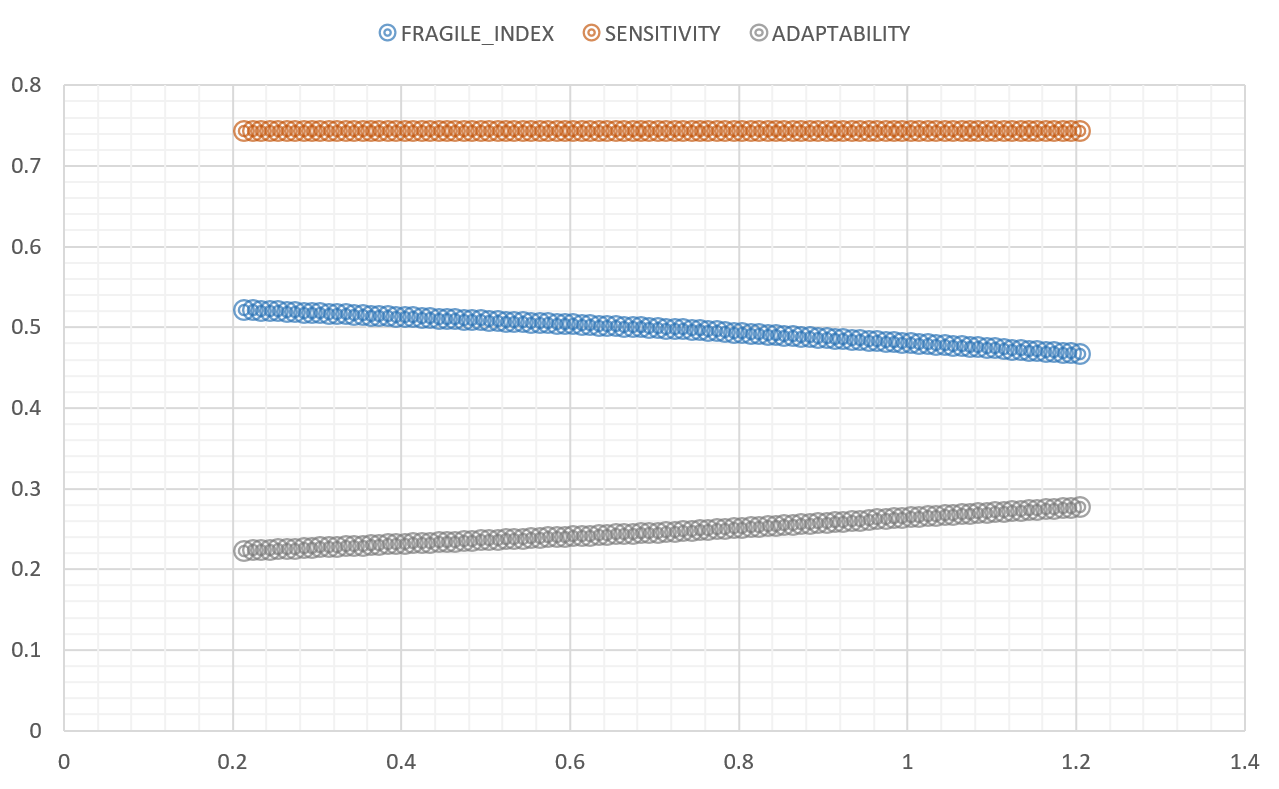
\includegraphics[width=10cm]{task4exp.png}
  \caption{relation between basic health services and sensibility}
  \label{fig:sanitation}
\end{figure}
\begin{table}[h]
  \centering
  \begin{tabular} {|c|c|c|c|c|c|c|}  
  \hline  
  Variable & GDP & FRE & GEF & FDS & BHS & STA \\ \hline  
  Weight & 0.43 & 0.12 & 0.22 & 0.12 & 0.22 & 0.61  \\ \hline  
  \end{tabular}  
  \caption{The weight of adaptability factors}
\end{table}
We can see from the table that the GDP per capita and the 
degree of government stability have a greater impact on 
national adaptability. People can prevent the country from 
becoming vulnerable because of climatic factors by strengthening 
the construction of these two aspects.

\subsection{Task V}
We try to enter the parameters of some larger countries and 
smaller countries into our model and find that our model yields 
a more accurate value for the fragility of larger countries. 
However, for some countries with very small land areas, the 
result of the model is not that good. Our improvement plans 
are as follows:
\begin{itemize}
  \item We can try using more training sample data to improve the model.
  \item We can increase the number of hidden layers in the model, but 
  this may lead to over-fitting.
  \item We can combine our existing BP Neural Network with genetic 
  algorithm and use genetic algorithm to tune the characteristic 
  parameters of BP Neural Network.
\end{itemize}
\begin{figure}[htbp]
  \centering
  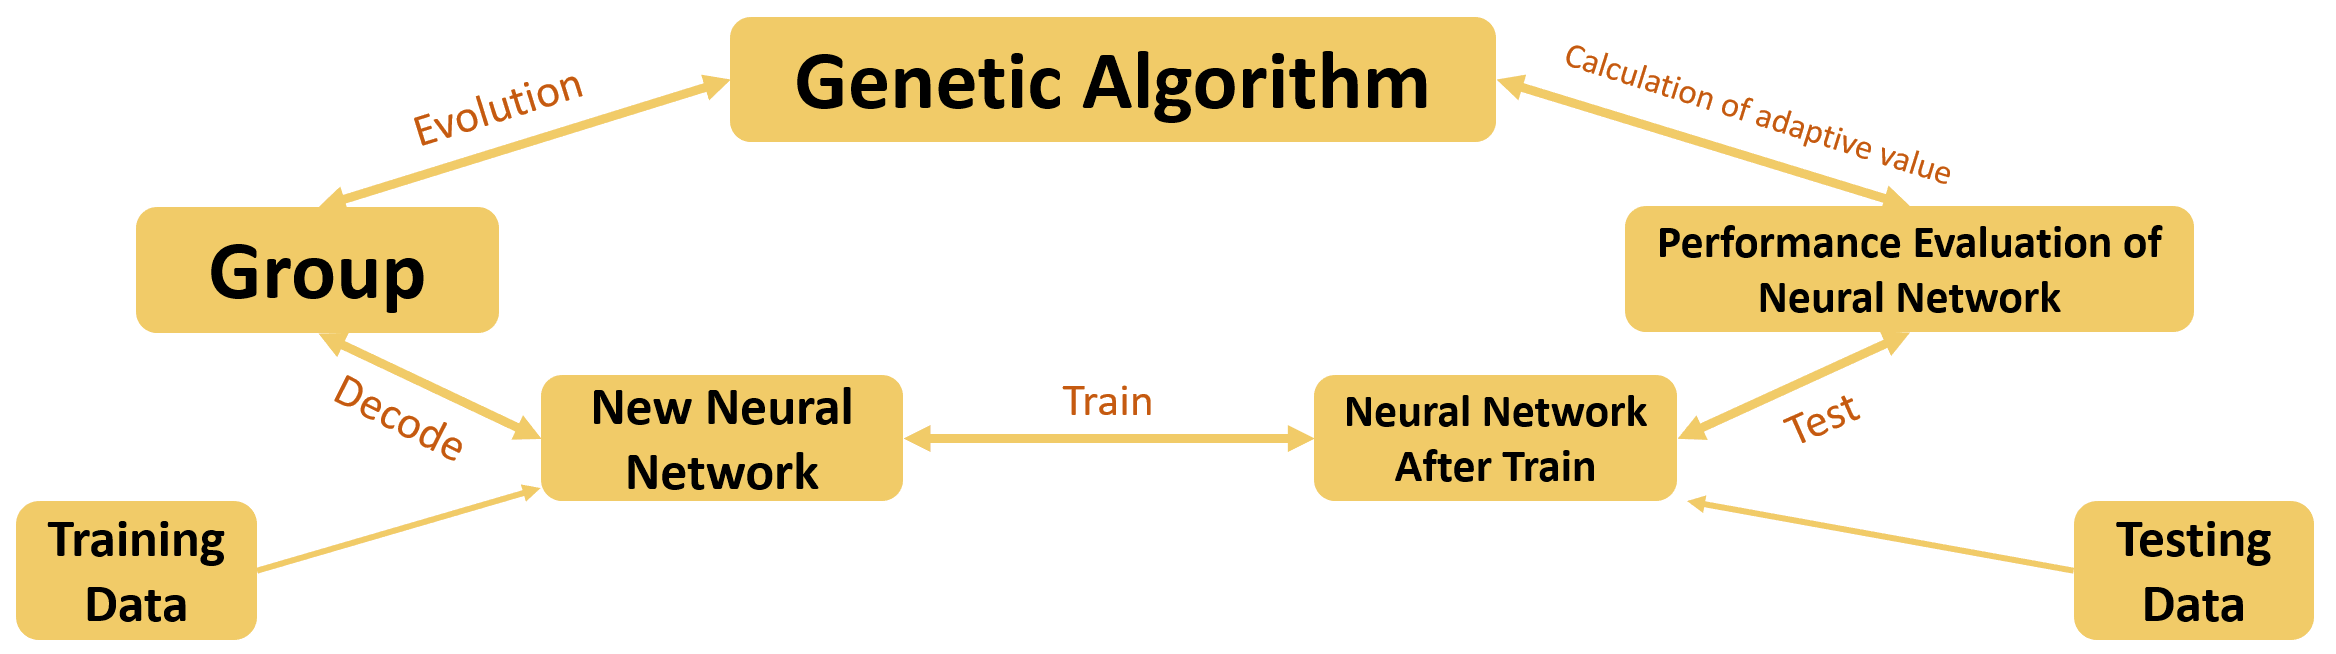
\includegraphics[width=12cm]{zaojia.png}
  \caption{Genetic Algorithm with BP Neural Network}
\end{figure}
\newgeometry{bottom=1cm}
\begin{table}[h]
  \linespread{1.0}
  \centering
  \caption{Comparison}
  \label{my-label}
  \setlength{\tabcolsep}{7mm}{
  \begin{tabular}{c|p{3cm}<{\centering}|p{3cm}<{\centering}}
  \shline
  \textbf{States} & \textbf{Accuracy(MSE) before improving} & \textbf{Accuracy(MSE) after improving}\\ \hline
  Somalia   & 0.08   & 0.19  \\ \hline
  Haiti   & 0.11   & 0.09            \\ \hline
  Zimbabwe   & 0.04   & 0.16         \\ \hline
  Monaco   & 0.03   & 0.05    \\ \hline
  Laos   & 0.07   & 0.14          \\ \hline
  India   & 0.06   & 0.10     \\ \hline
  Australia   & 0.07   & 0.08                            \\ \hline
  Brazil   & 0.03   & 0.08          \\ \hline
  Russia   & 0.07   & 0.09           \\ \shline
  \end{tabular}}
  \end{table} 
  % \newpage
  As can be seen from the table, the accuracy improved after the optimization of genetic algorithm.





\section{Strengths and Weaknesses}
\subsection{Strengths of Models}
\begin{itemize}
  \item \textbf{Inclusive:} Our model contains two large indicators (sensitivity and adaptability), and 
  considers of the state's ability to intervene in natural factors such as climate. 
  Our model incorporates all aspects of the fragility index. The small indicators 
  in the two big indexes(sensitivity and adaptability) are composed of various political, 
  economic, climate, social and cohesion sectors.
  \item \textbf{Quantification:} Our model can output a numerical value to quantify the fragility of a country. 
  The use of Numbers is more intuitive and more conducive to contrast, which can clearly 
  reflect changes of the fragility when input parameters change.
  \item \textbf{Simple but Universal:} We use the neural network model, which is relatively simple, also does not break 
  generality. If there is enough training data, each country's fragility index 
  can be figured out  accurate.
  \item \textbf{Visible and Understandable:} We used the plotly library of python to present the model and data 
  intuitively in the form of line graphs, which is more visualized and 
  easier to understand.
\end{itemize}


\subsection{Weaknesses of Models}
\begin{itemize}
  \item \textbf{Accuracy Relies on Statistics:} The accuracy of our model 
  depends not only on the reliability of the data itself, but also on the 
  number of training data. The more the training data has, 
  the more accurate the model is.
  \item \textbf{Not a long-term and dynamic model:} Our model is a static 
  model focusing on short-term changes. But, on the contrast, the factors 
  that affect fragility are long-term, dynamic and highly uncertain. 
  In terms of long-term time scale, we need to focus on future risks, and 
  we need to consider the dynamic assessment framework that changes with time. 
\end{itemize}
\restoregeometry

% 图文混排
% \begin{wrapfigure}{l}{4.5cm}%靠文字内容的左侧
%   
\includegraphics[width=4cm]{test1.jpg}\\
%   \caption{Podala Palace, Tibet}\label{fig:tibet}
%   \end{wrapfigure}

% 论文引用
\newpage
\begin{thebibliography}{99}
\bibitem{bib1} water dependency ratio, The World Bank, \\ 
https://data.worldbank.org/indicator/AG.LND.PRCP.MM?name\_desc=false, 
2017.
\bibitem{bib2} Droughts, floods, extreme temperatures (\% of 
population, average 1990-2009), The World Bank, 
https://data.worldbank.org/indicator/EN.CLC.MDAT.ZS, 1990-2009.
\bibitem{bib3} Global Climate Risk Index, The World Bank,\\
http://search.worldbank.org/data?qterm=climate+change\&language=\&format=,
\\viewed 7th January, 2016.
\bibitem{bib4} DEATH RATE, "The World Factbook". Cia.gov, 
\\https://www.cia.gov/library/publications/the-world-factbook/rankorder/2066rank.html,\\ 
Retrieved 2014-02-21.
\bibitem{bib5} Global Food Security Index, Food Security Index, viewed 2nd February, 2016, foodsecurityindex.eiu.com.
\bibitem{bib6} Most Dangerous Countries in the World, ATLAS \& BOOTS,\\ 
https://www.atlasandboots.com/most-dangerous-countries-in-the-world-ranked/, \\
viewed 29th January, 2017.
\bibitem{bib7} Basic Health Services by Country, www.worldmapper.org, \\
http://www.worldmapper.org/display.php?selected=220, viewed 1st August, 2016.
\bibitem{bib8} Zhang qian;Meng huixin. Social fragility and 
poverty under the influence of climate change: a review of foreign studies. 
Journal of agricultural university of China (social science edition), 2014, 31.2: 56-67.
\bibitem{bib9} Current World Death Rate, The World Factbook 2012,\\ 
https://www.cia.gov/library/publications/the-world-factbook/rankorder/2066rank.html, \\
viewed 27th November, 2012.
\bibitem{bib10} Refugee population by country or territory of origin, https://data.worldbank.org.
\bibitem{bib11} A. Alesina, E. La Ferrara (2005). Ethnic Diversity and Economic 
Performance. Journal of Economic Literature: 762–800. Retrieved December 15, 2016.
\bibitem{bib12} GDP per capita (current US\$),The World Bank. Accessed on 26 December 
2016, Liechtenstein updated 6. November 2016.
\bibitem{bib13} Global Hunger Index, International Food Policy Research Institute 
(IFPRI) 2011, Global Hunger Index - 2011,
http://www.ifpri.org/publication/2011-global-hunger-index, \\ 
viewed 17th October, 2011.
\bibitem{bib14} Freedom in the World 2017, freedomhouse.org,\\ 
https://freedomhouse.org/report/freedom-world/freedom-world-2017, \\ 
viewed 15th September, 2017.
\bibitem{bib15} Global FirePower Index, GFP,
http://www.globalfirepower.com/countries-listing.asp, \\ 
viewed 15th February, 2016.
\bibitem{bib16} Government Effectiveness, The Worldwide Governance 
Indicators (WGI) project, The World Bank Group, 
http://info.worldbank.org/governance/wgi/index.asp, viewed 21st October, 2011.
\bibitem{bib17} Political Stability and Absence of Violence/Terrorism, 
The Worldwide Governance Indicators (WGI) project, The World Bank Group, \\
http://info.worldbank.org/governance/wgi/index.asp, viewed 21st October, 2011.
\bibitem{bib18} Cutter S L, Boruff B J, Shirley W L. Social 
Fragility to Environmental Hazards. Social Science 
Quarterly, 2003, 84: 242 - 261.
\bibitem{bib19} O’Brien K, Eriksen S, Schjolen A, et al. What’s in a Word?, 
Conflicting Interpretations of fragility in Climate Change Research. CICERO Working Paper, 2004(4)
\bibitem{bib20} matlab neural network 30 case analysis, Matlab Chinese BBS, Beijing: Beijing aerospace university press, 2010.
\end{thebibliography}

% 附录
\begin{appendices}

\section{Code}

\textbf{\textcolor[rgb]{0.98,0.00,0.00}{Input python source:}}
\lstinputlisting[language=Python]{./code/code.py}

\section{Data}
\begin{figure}[htbp]
  \centering
  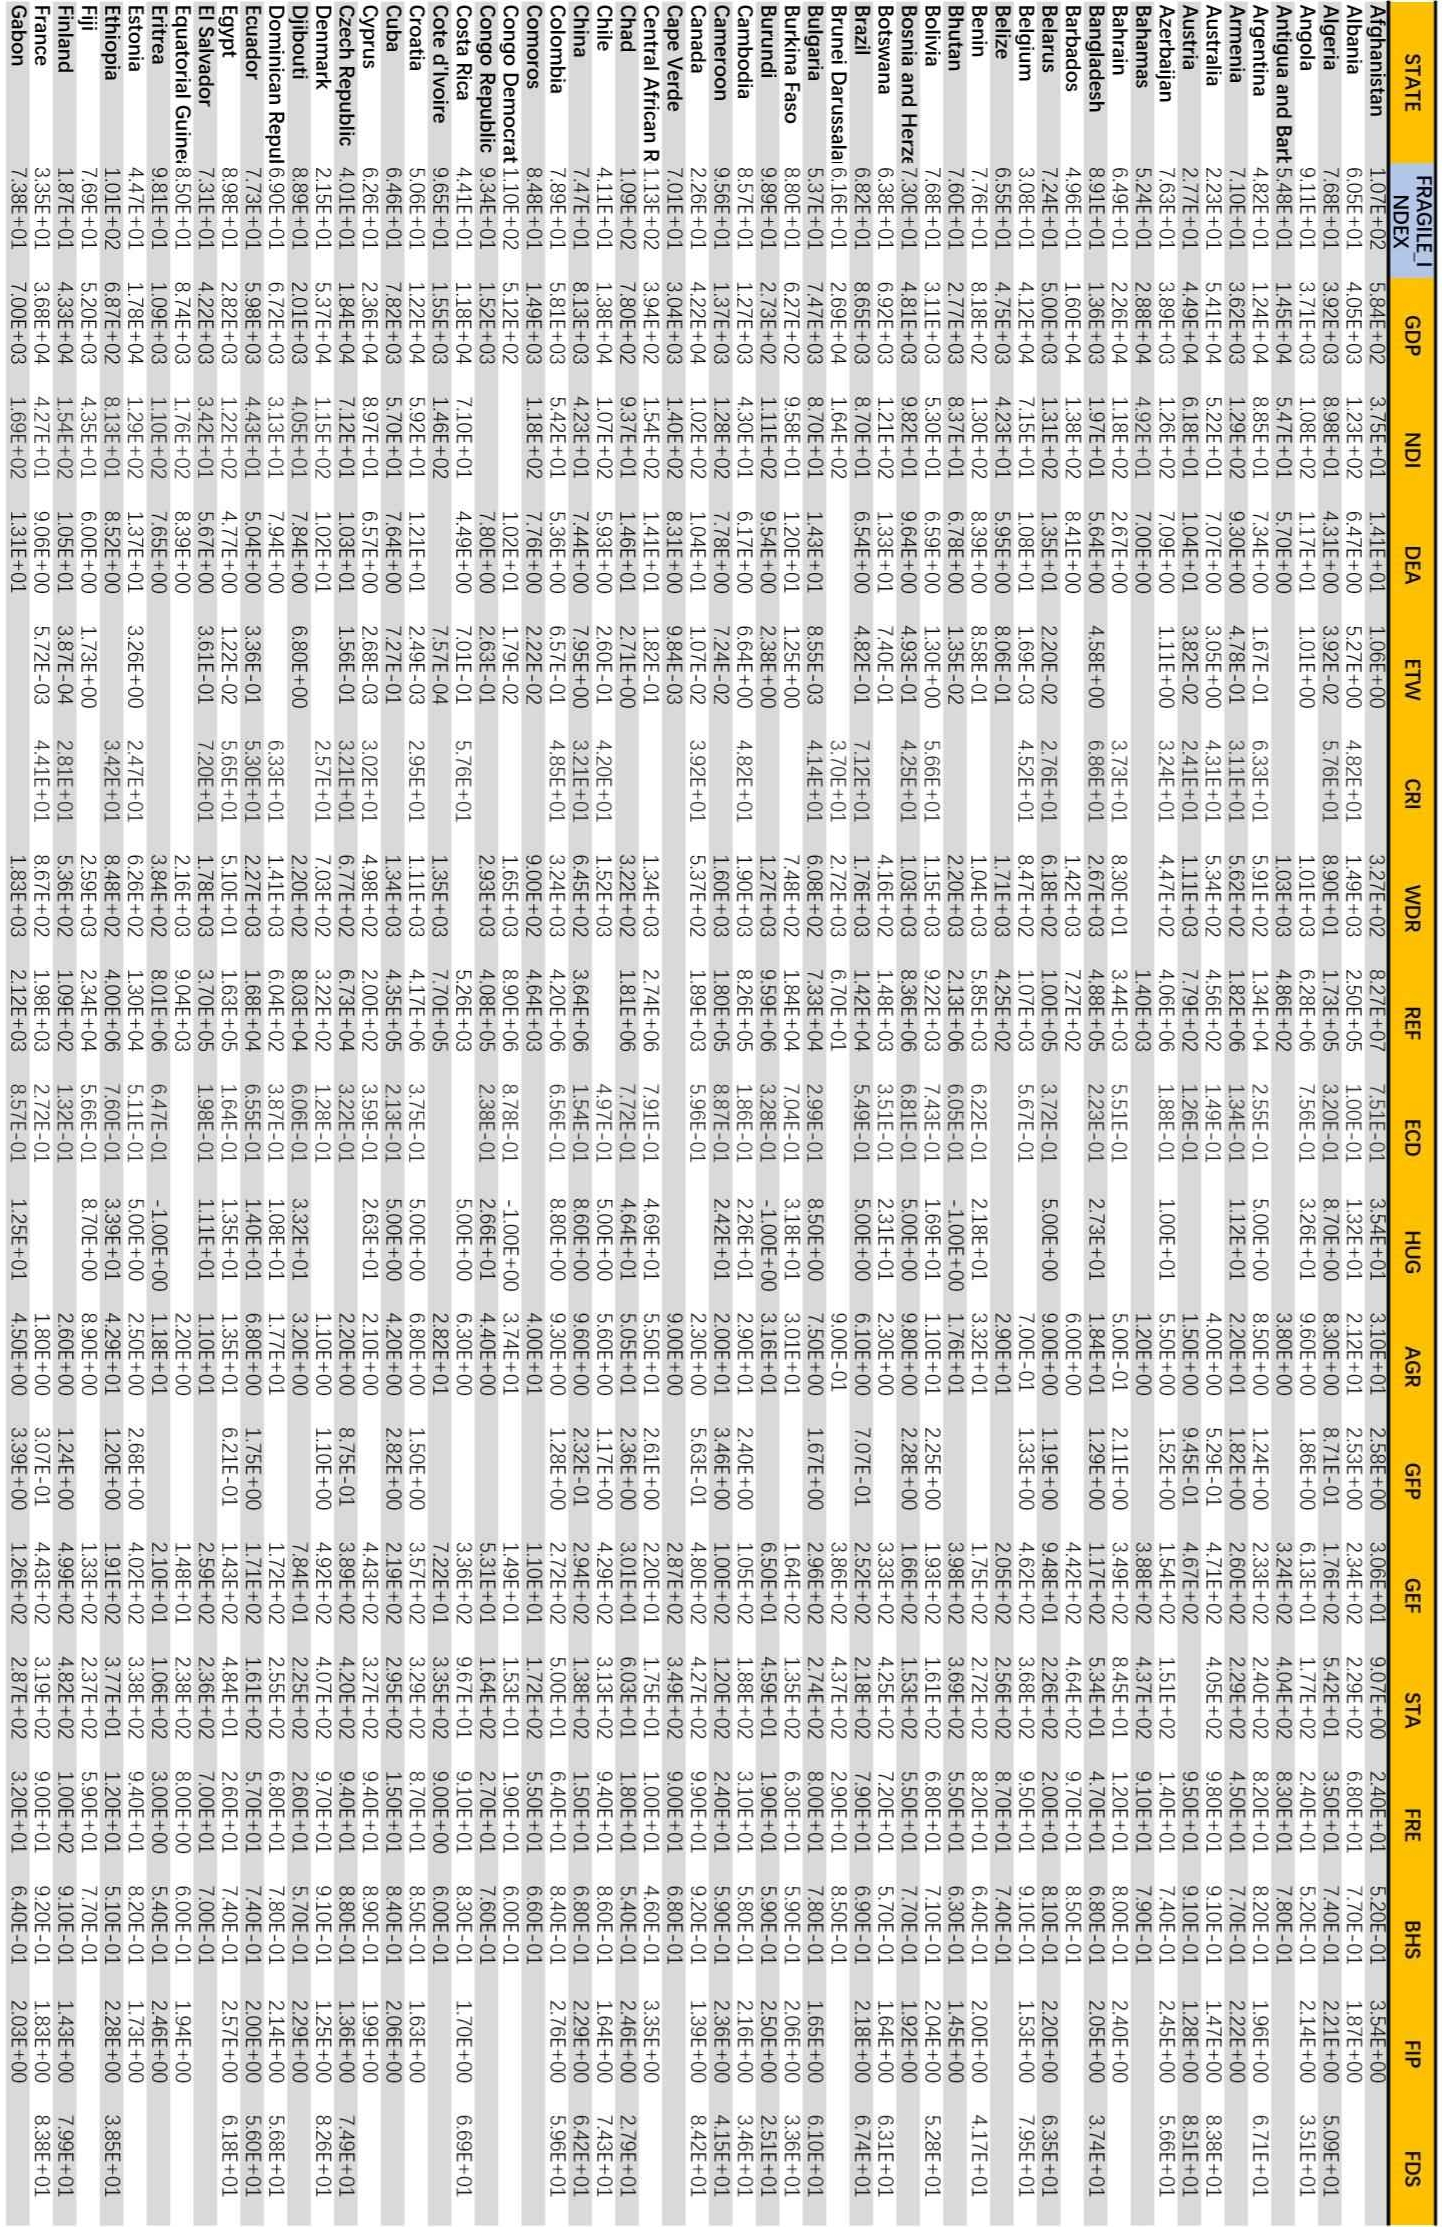
\includegraphics[width=15cm]{data1.jpg}
\end{figure}
\begin{figure}[htbp]
  \centering
  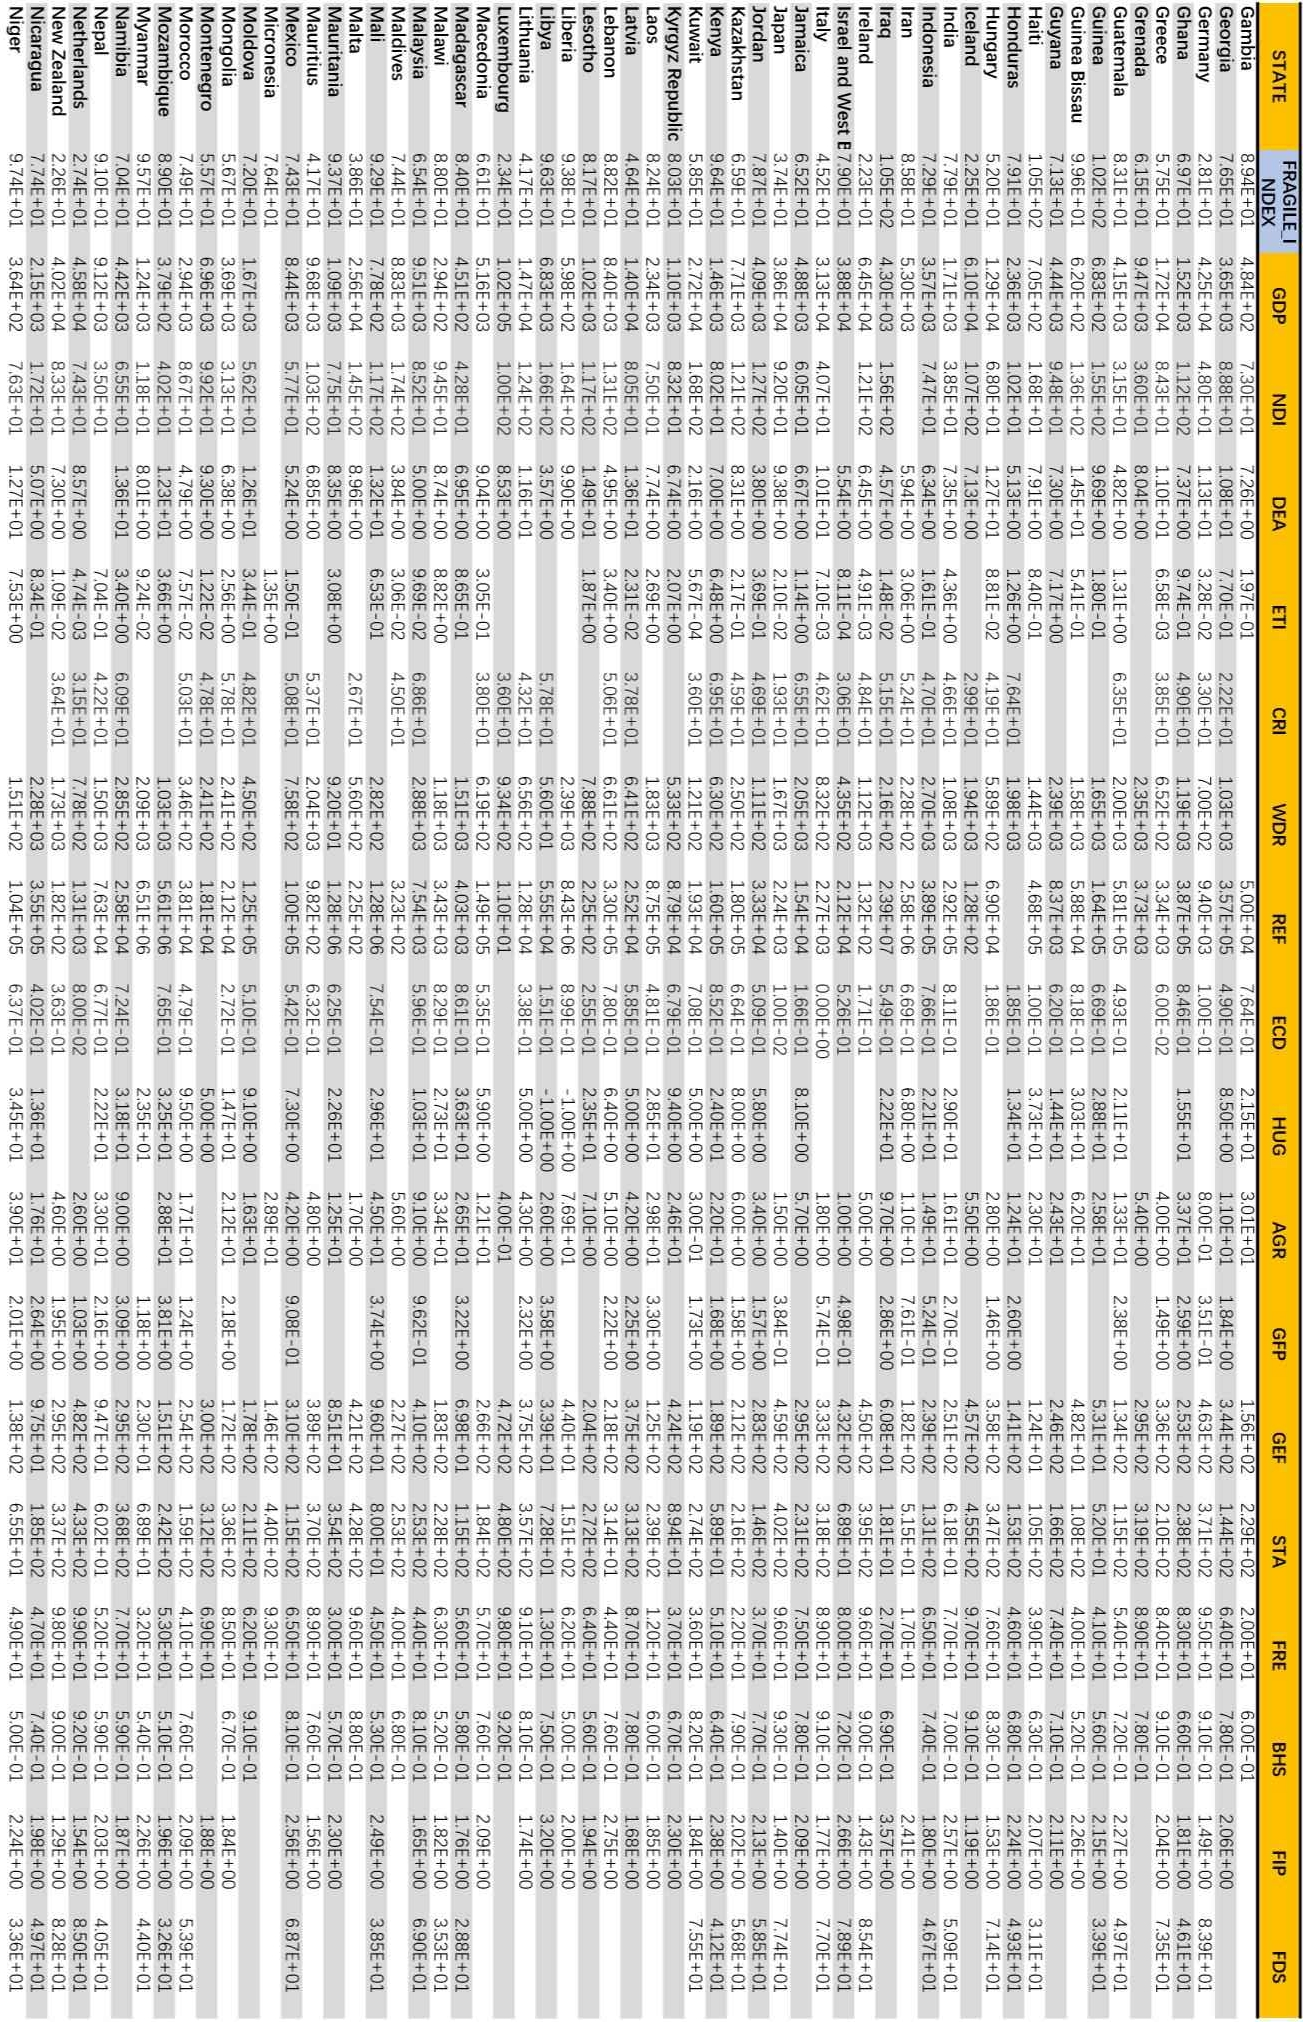
\includegraphics[width=15cm]{data2.jpg}
\end{figure}
\begin{figure}[htbp]
  \centering
  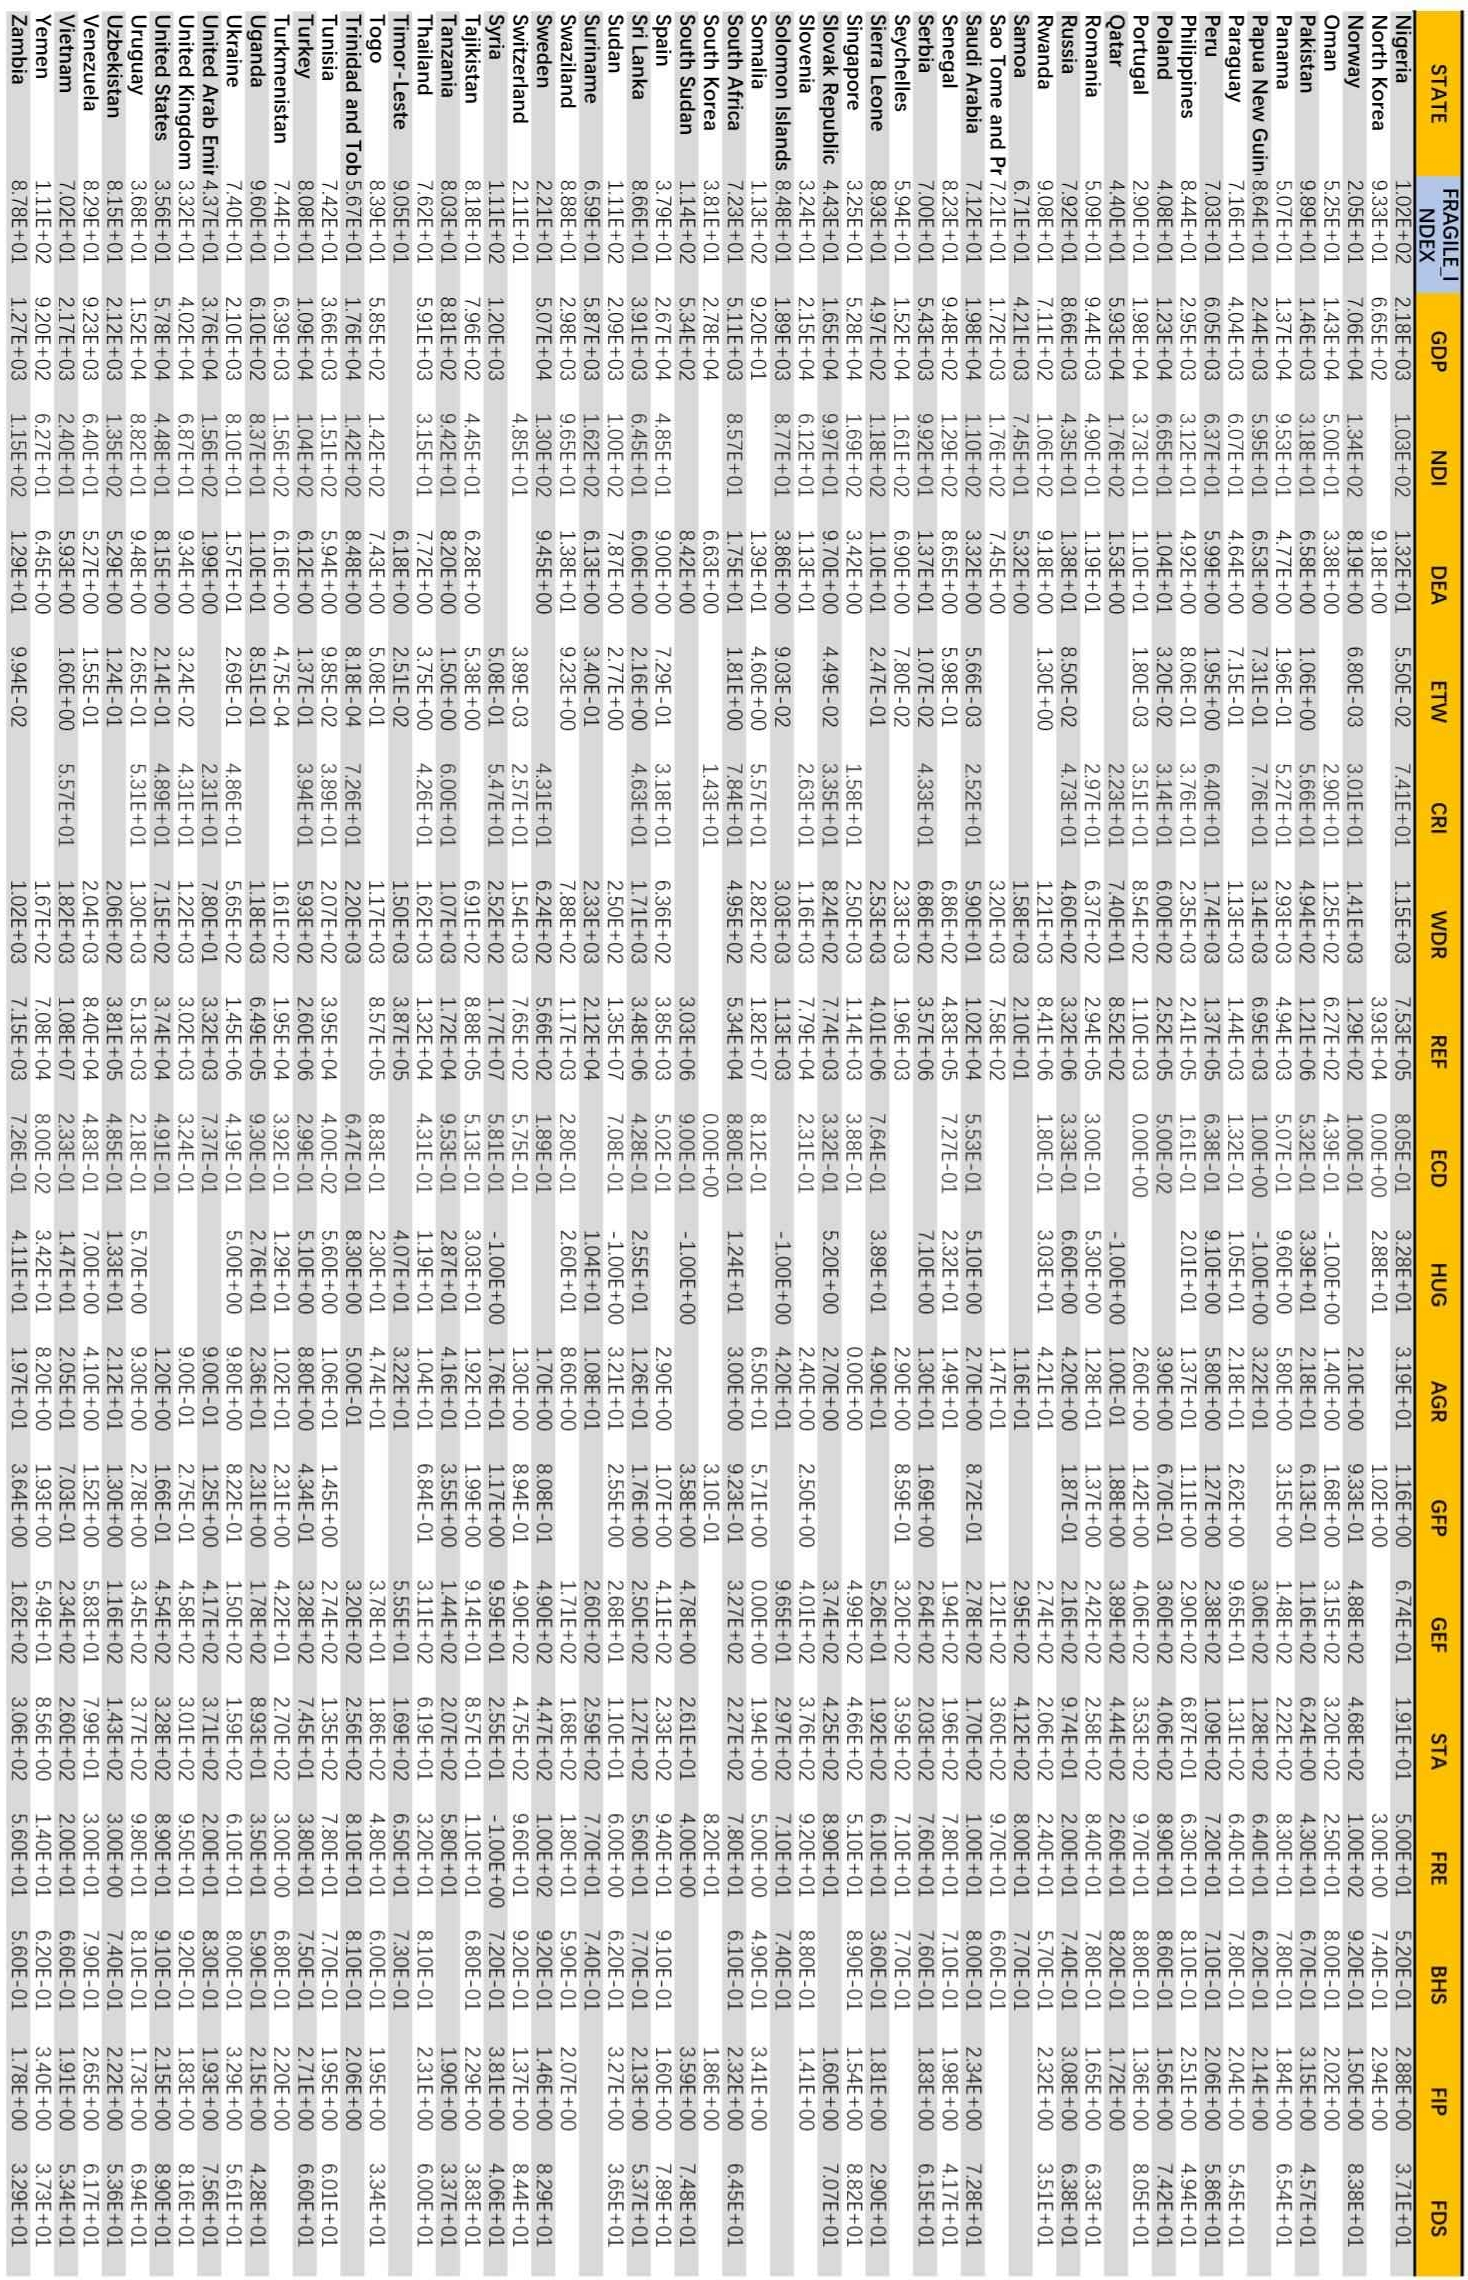
\includegraphics[width=15cm]{data3.jpg}
\end{figure}
\newpage
\section{Training Process}
\begin{figure}[htbp]
  \centering
  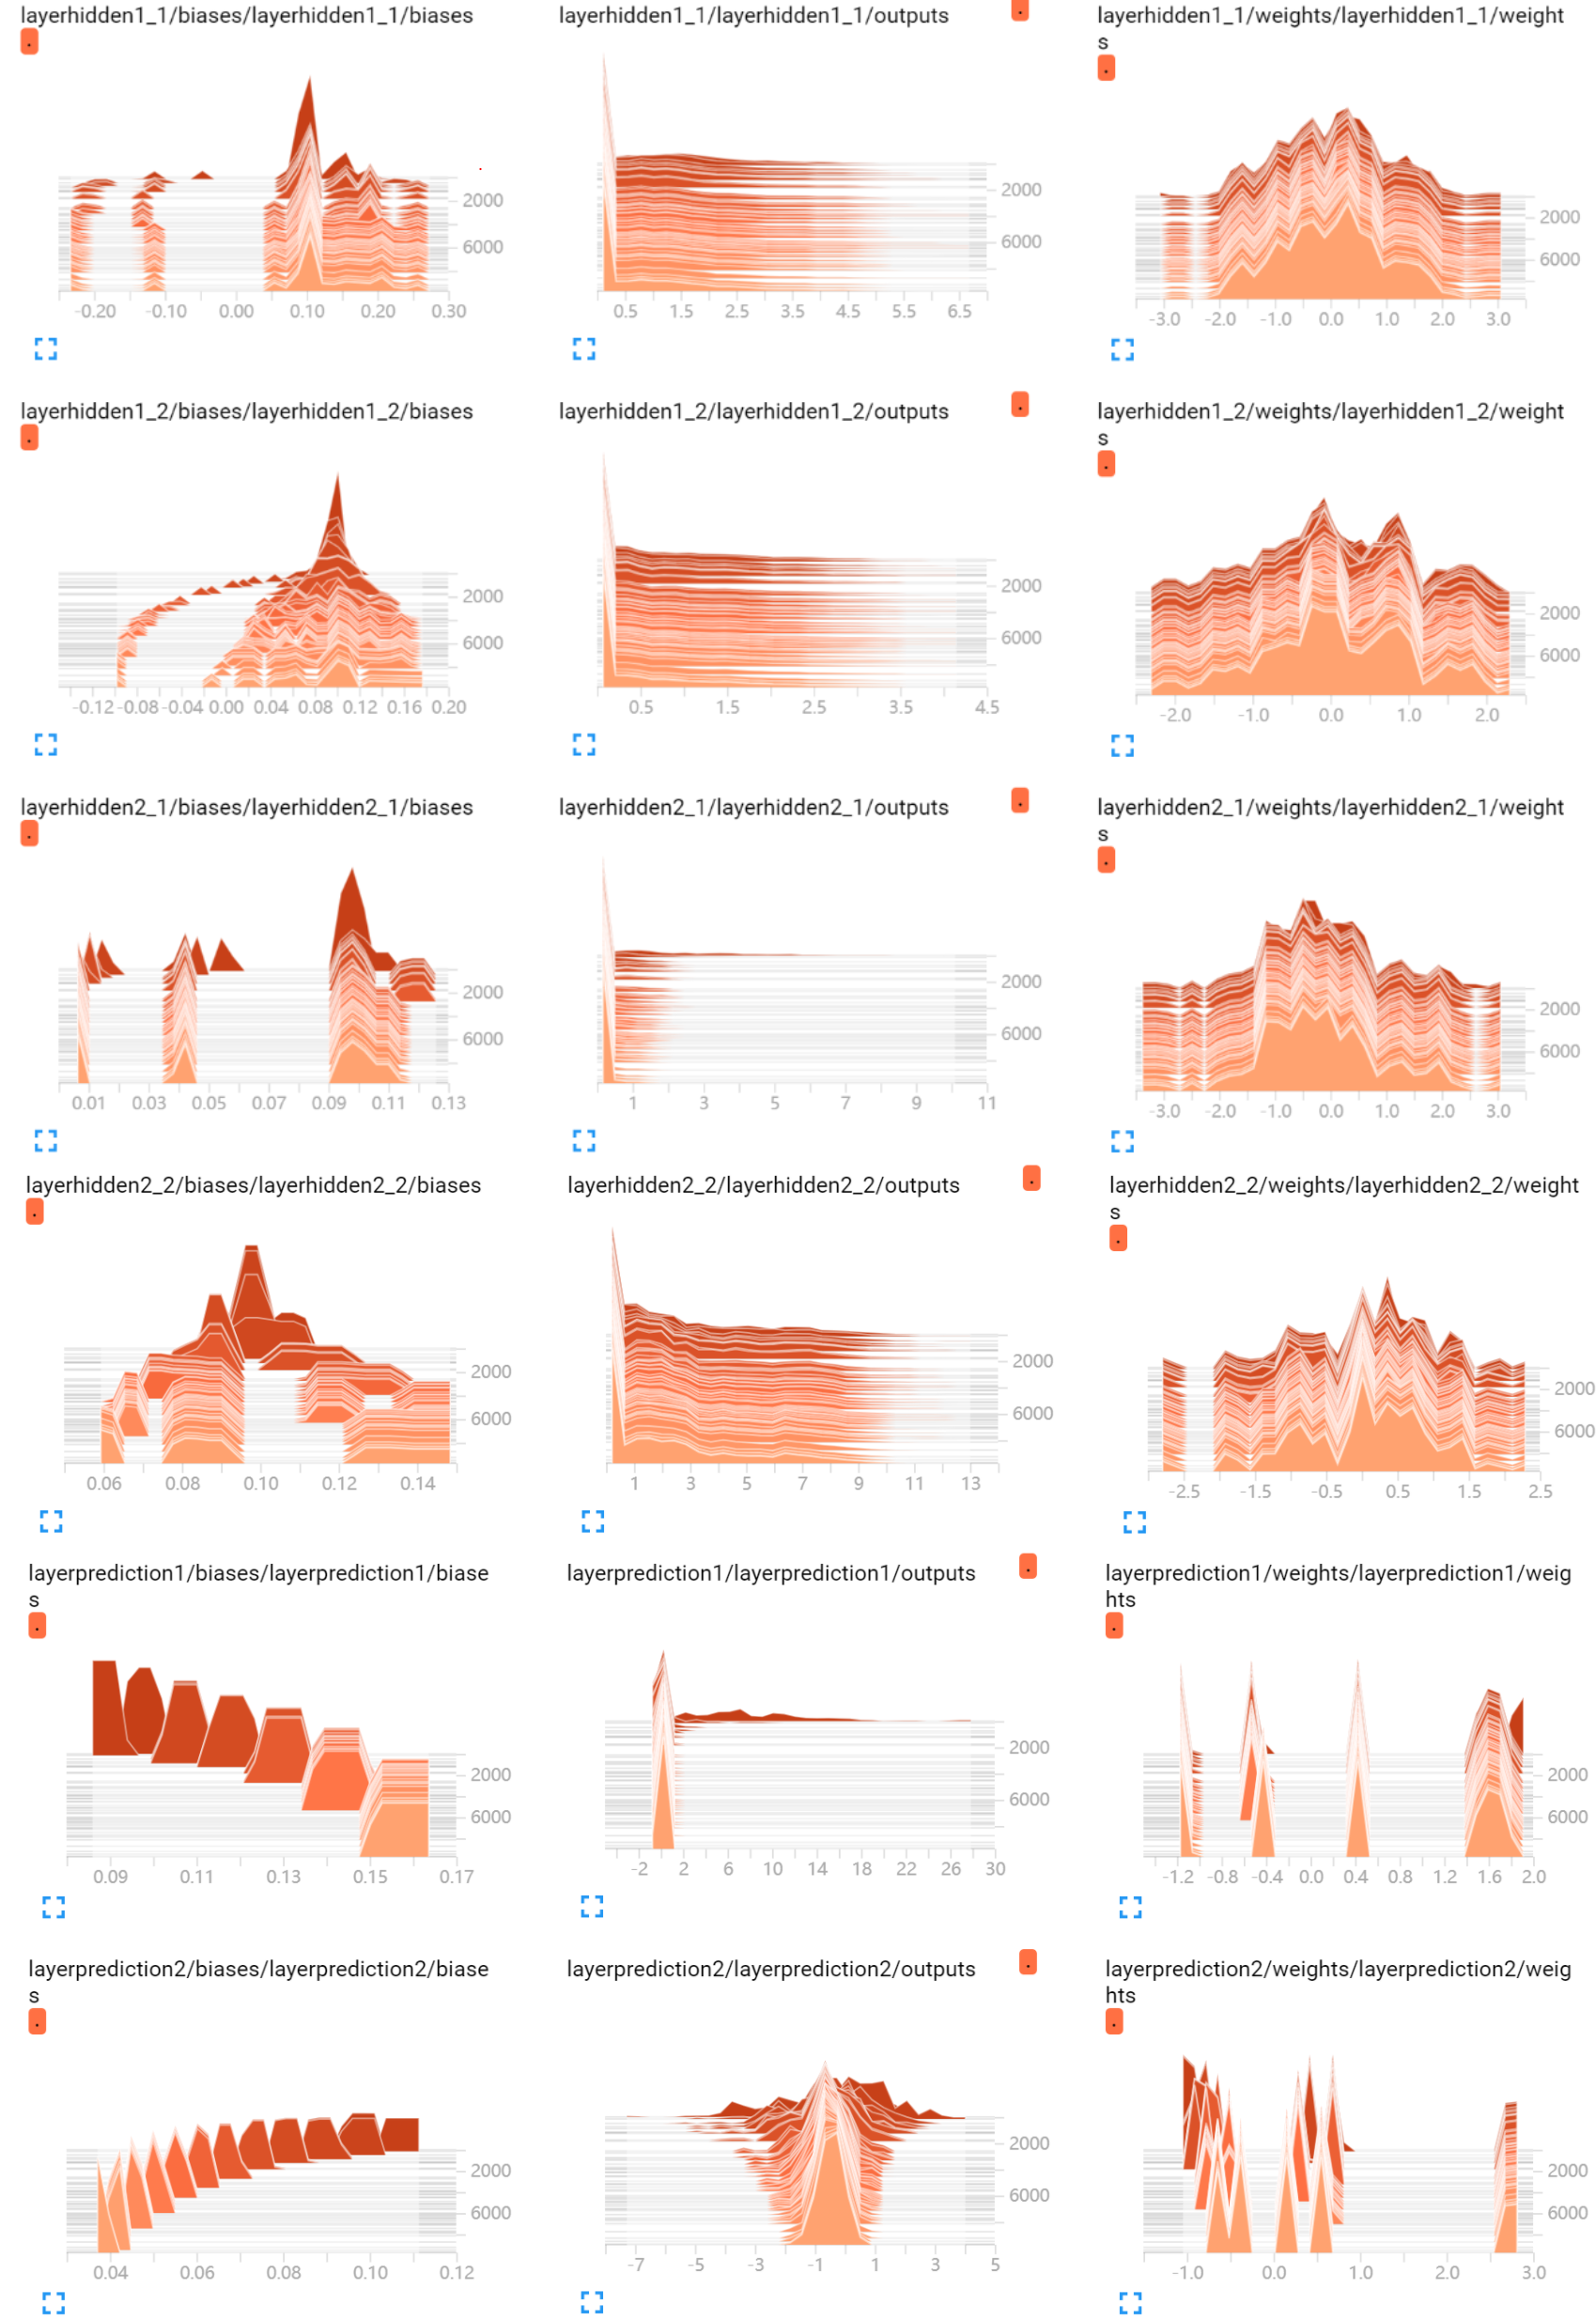
\includegraphics[width=14cm]{training.png}
\end{figure}
\end{appendices}
\end{document}


%% 
%% This work consists of these files mcmthesis.dtx,
%%                                   figures/ and
%%                                   code/,
%% and the derived files             mcmthesis.cls,
%%                                   mcmthesis-demo.tex,
%%                                   README,
%%                                   LICENSE,
%%                                   mcmthesis.pdf and
%%                                   mcmthesis-demo.pdf.
%%
%% End of file `mcmthesis-demo.tex'.
